%% BioMed_Central_Tex_Template_v1.06
%%                                      %
%  bmc_article.tex            ver: 1.06 %
%                                       %

%%IMPORTANT: do not delete the first line of this template
%%It must be present to enable the BMC Submission system to
%%recognise this template!!

%%%%%%%%%%%%%%%%%%%%%%%%%%%%%%%%%%%%%%%%%
%%                                     %%
%%  LaTeX template for BioMed Central  %%
%%     journal article submissions     %%
%%                                     %%
%%          <8 June 2012>              %%
%%                                     %%
%%                                     %%
%%%%%%%%%%%%%%%%%%%%%%%%%%%%%%%%%%%%%%%%%


%%%%%%%%%%%%%%%%%%%%%%%%%%%%%%%%%%%%%%%%%%%%%%%%%%%%%%%%%%%%%%%%%%%%%
%%                                                                 %%
%% For instructions on how to fill out this Tex template           %%
%% document please refer to Readme.html and the instructions for   %%
%% authors page on the biomed central website                      %%
%% http://www.biomedcentral.com/info/authors/                      %%
%%                                                                 %%
%% Please do not use \input{...} to include other tex files.       %%
%% Submit your LaTeX manuscript as one .tex document.              %%
%%                                                                 %%
%% All additional figures and files should be attached             %%
%% separately and not embedded in the \TeX\ document itself.       %%
%%                                                                 %%
%% BioMed Central currently use the MikTex distribution of         %%
%% TeX for Windows) of TeX and LaTeX.  This is available from      %%
%% http://www.miktex.org                                           %%
%%                                                                 %%
%%%%%%%%%%%%%%%%%%%%%%%%%%%%%%%%%%%%%%%%%%%%%%%%%%%%%%%%%%%%%%%%%%%%%

%%% additional documentclass options:
%  [doublespacing]
%  [linenumbers]   - put the line numbers on margins

%%% loading packages, author definitions

%\documentclass[twocolumn]{bmcart}% uncomment this for twocolumn layout and comment line below
\documentclass{bmcart}

%%% Load packages
%\usepackage{amsthm,amsmath}
%\RequirePackage{natbib}
%\RequirePackage[authoryear]{natbib}% uncomment this for author-year bibliography
%\RequirePackage{hyperref}
\usepackage[utf8]{inputenc} %unicode support
%\usepackage[applemac]{inputenc} %applemac support if unicode package fails
%\usepackage[latin1]{inputenc} %UNIX support if unicode package fails
\usepackage{todonotes}
\usepackage{multirow}
\usepackage{nameref}
\usepackage{amsmath}
\usepackage{hyperref}
\usepackage[table,xcdraw]{xcolor}
\usepackage{threeparttable}
\usepackage{subfig}
\usepackage[normalem]{ulem}
\usepackage{tikz}
\def\checkmark{\tikz\fill[scale=0.4](0,.35) -- (.25,0) -- (1,.7) -- (.25,.15) -- cycle;} 
\useunder{\uline}{\ul}{}


%%%%%%%%%%%%%%%%%%%%%%%%%%%%%%%%%%%%%%%%%%%%%%%%%
%%                                             %%
%%  If you wish to display your graphics for   %%
%%  your own use using includegraphic or       %%
%%  includegraphics, then comment out the      %%
%%  following two lines of code.               %%
%%  NB: These line *must* be included when     %%
%%  submitting to BMC.                         %%
%%  All figure files must be submitted as      %%
%%  separate graphics through the BMC          %%
%%  submission process, not included in the    %%
%%  submitted article.                         %%
%%                                             %%
%%%%%%%%%%%%%%%%%%%%%%%%%%%%%%%%%%%%%%%%%%%%%%%%%


% \def\includegraphic{}
% \def\includegraphics{}



%%% Put your definitions there:
\startlocaldefs
\endlocaldefs


%%% Begin ...
\begin{document}

%%% Start of article front matter
\begin{frontmatter}

\begin{fmbox}
\dochead{Research}

%%%%%%%%%%%%%%%%%%%%%%%%%%%%%%%%%%%%%%%%%%%%%%
%%                                          %%
%% Enter the title of your article here     %%
%%                                          %%
%%%%%%%%%%%%%%%%%%%%%%%%%%%%%%%%%%%%%%%%%%%%%%

\title{Machine learning approach for predicting miRNA targets across organisms}    

\todo{The title should be changed -- we do not offer here an approach yet, but rather an analysis}
%%%%%%%%%%%%%%%%%%%%%%%%%%%%%%%%%%%%%%%%%%%%%%
%%                                          %%
%% Enter the authors here                   %%
%%                                          %%
%% Specify information, if available,       %%
%% in the form:                             %%
%%   <key>={<id1>,<id2>}                    %%
%%   <key>=                                 %%
%% Comment or delete the keys which are     %%
%% not used. Repeat \author command as much %%
%% as required.                             %%
%%                                          %%
%%%%%%%%%%%%%%%%%%%%%%%%%%%%%%%%%%%%%%%%%%%%%%

\author[
   addressref={aff1},                   % id's of addresses, e.g. {aff1,aff2}
   corref={aff1},                       % id of corresponding address, if any
   noteref={n1},                        % id's of article notes, if any
   email={benorgi@post.bgu.ac.il}   % email address
]{\inits{GBO}\fnm{Gilad} \snm{Ben Or}}

\author[
 addressref={aff2},
  corref={aff2},                       % id of corresponding address, if any
   noteref={n2},                        % id's of article notes, if any
   email={vaksler@post.bgu.ac.il}
]{\inits{IVL}\fnm{Isana} \snm{Veksler-Lublinsky}}

%%%%%%%%%%%%%%%%%%%%%%%%%%%%%%%%%%%%%%%%%%%%%%
%%                                          %%
%% Enter the authors' addresses here        %%
%%                                          %%
%% Repeat \address commands as much as      %%
%% required.                                %%
%%                                          %%
%%%%%%%%%%%%%%%%%%%%%%%%%%%%%%%%%%%%%%%%%%%%%%

\address[id=aff1]{%                           % unique id
  \orgname{Department of Information Systems Engineering, Ben-Gurion University of the Negev}, % university, etc
%   \street{Waterloo Road},                     %
  %\postcode{}                                % post or zip code
  \city{Beer Sheva},                              % city
  \cny{Israel}                                    % country
}


\address[id=aff2]{%                           % unique id
  \orgname{Department of Information Systems Engineering, Ben-Gurion University of the Negev}, % university, etc
%   \street{Waterloo Road},                     %
  %\postcode{}                                % post or zip code
  \city{Beer Sheva},                              % city
  \cny{Israel}                                    % country
}



% \address[id=aff2]{%
%   \orgname{Marine Ecology Department, Institute of Marine Sciences Kiel},
%   \street{D\"{u}sternbrooker Weg 20},
%   \postcode{24105}
%   \city{Kiel},
%   \cny{Germany}
% }

%%%%%%%%%%%%%%%%%%%%%%%%%%%%%%%%%%%%%%%%%%%%%%
%%                                          %%
%% Enter short notes here                   %%
%%                                          %%
%% Short notes will be after addresses      %%
%% on first page.                           %%
%%                                          %%
%%%%%%%%%%%%%%%%%%%%%%%%%%%%%%%%%%%%%%%%%%%%%%

\begin{artnotes}
%\note{Sample of title note}     % note to the article
\note[id=n1]{Equal contributor} % note, connected to author
\end{artnotes}

\end{fmbox}% comment this for two column layout

%%%%%%%%%%%%%%%%%%%%%%%%%%%%%%%%%%%%%%%%%%%%%%
%%                                          %%
%% The Abstract begins here                 %%
%%                                          %%
%% Please refer to the Instructions for     %%
%% authors on http://www.biomedcentral.com  %%
%% and include the section headings         %%
%% accordingly for your article type.       %%
%%                                          %%
%%%%%%%%%%%%%%%%%%%%%%%%%%%%%%%%%%%%%%%%%%%%%%

\begin{abstractbox}

\begin{abstract} % abstract
\parttitle{Background}
Machine learning models achieve high accuracy score in miRNA-target prediction of human cells. The models tries to identify rules for interaction between the miRNAs and the targets. There are variety of statistical and deep learning models, which use either high-level or raw-level features. The recent researches tried to improve the performance of the models by suggesting better model architecture or better feature engineering. In this paper, we move the focus to the data: We collected 8 high throughput miRNA-target chimeras datasets of human, mouse, celegans and cattle from a variety of sources. We assumed that this is possible to adopt/ transfer rules from one organism to other. We use our dataset collection for both in-organism and intra-organism target prediction and verify our assumptions.

\parttitle{Results}
For human target prediction, the xGBoost model achieved the same performance as the latest published target prediction models. It achieved high accuracy score in predict the rest of the datsets as well. We show that it is possible to predict an oranisim based on a model trained on different organism. However, the prediction performance depends on vairety of paramters such as evolutionary distance, the tissue which was examined, the degree of similarity between the datasets, the datasets size and etc.

\parttitle{Conclusions}
Our research finds that there rules that can be adopt from one organism to other. The strength of the rules and the ability to use them depends especially on the distance between the organisims.  Our first comprehensive unified collection of CLASH datasets enable us to examine and compare the ability to learn from one organism to another. In the future it also will enable to improve predication score based on techniques such as transfer learning.


\end{abstract}

%%%%%%%%%%%%%%%%%%%%%%%%%%%%%%%%%%%%%%%%%%%%%%
%%                                          %%
%% The keywords begin here                  %%
%%                                          %%
%% Put each keyword in separate \kwd{}.     %%
%%                                          %%
%%%%%%%%%%%%%%%%%%%%%%%%%%%%%%%%%%%%%%%%%%%%%%

\begin{keyword}
\kwd{sample}
\kwd{article}
\kwd{author}
\end{keyword}

% MSC classifications codes, if any
%\begin{keyword}[class=AMS]
%\kwd[Primary ]{}
%\kwd{}
%\kwd[; secondary ]{}
%\end{keyword}

\end{abstractbox}
%
%\end{fmbox}% uncomment this for twcolumn layout

\end{frontmatter}

%%%%%%%%%%%%%%%%%%%%%%%%%%%%%%%%%%%%%%%%%%%%%%
%%                                          %%
%% The Main Body begins here                %%
%%                                          %%
%% Please refer to the instructions for     %%
%% authors on:                              %%
%% http://www.biomedcentral.com/info/authors%%
%% and include the section headings         %%
%% accordingly for your article type.       %%
%%                                          %%
%% See the Results and Discussion section   %%
%% for details on how to create sub-sections%%
%%                                          %%
%% use \cite{...} to cite references        %%
%%  \cite{koon} and                         %%
%%  \cite{oreg,khar,zvai,xjon,schn,pond}    %%
%%  \nocite{smith,marg,hunn,advi,koha,mouse}%%
%%                                          %%
%%%%%%%%%%%%%%%%%%%%%%%%%%%%%%%%%%%%%%%%%%%%%%
\section*{Introduction}


\subsection*{miRNAs summary}
miRNAs are small non-coding RNAs that regulate gene expression post-transcriptionally. The functional mature miRNAs are generated in a multi-stage process (Ref 1), and are eventually associate with Argonaute proteins to form the core of the miRNA-induced silencing complex (miRISC). miRISC uses the sequence information in the miRNA as a guide to bind complementary sequences on mRNAs, which leads to repression of translation and/or mRNA degradation. MiRNAs function in diverse aspects of development and physiology and have been implicated in human disease (Ref 2). After their discovery in Caenorhabditis elegans (C. elegans) in 1993 (Ref 3, 4), miRNAs were shown to be present in all animals and plants and in many viruses (Ref 5).

\subsection*{Identification of miRNA-target interactions}
Identification of miRNA target sites on mRNAs is a fundamental step in understanding miRNA function.

\subsubsection*{Experimental identification}

Experimental identification of target genes which is not direct

Give examples and limitations

From deepMirTar:
Traditionally, experimental biochemical assays, such as reporter assays, western blot, quantitative polymerase chain reaction, microarrays and next-generation sequencing (NGS), can identify miRNA targets.

Drawback:
One drawback of these methods is that the targets are identified at the gene level, making it difficult to locate the exact miRNA-binding site on the mRNA (Menor et al., 2014)

AGO-CLIP methods - site of interaction is known, however the exact miRNA-target pair is not.

\todo{read the Zefat paper}

CLASH methods:
In the past few years, several high-throughput methods that can capture miRNAs bound to their respective targets have been developed (Refs 24-27). These methods are derived from Argonaute cross‐linking and immunoprecipitation (AGO‐CLIP) and use an extra step to covalently ligate the miRNA and the target RNA. Subsequent cloning and sequencing of isolated RNAs capture short chimeric miRNA‐target reads which facilitates the identification of specific miRNA‐target interactions. An additional method iCLIP (28) that was applied in C. elegans reported a recovery of chimera sequences without an additional ligation step with similar efficiency to the methods above.

Note - not only in C.elegans spontaneous linking was observed.

 Experimental identification is laborious and time-consuming; high-throughput miRNA-target interactions datasets are available only for a small number of model organisms. 

\subsubsection*{Computational prediction}

From deepMirTar: 
The costly and time-consuming experimental identification of
miRNA targets promotes reliance on computational tools to predict
a set of credible target candidates for further experimental validation.

Computational identification is also very challenging, since miRNAs are short and engage only limited sequence complementarity to their targets. 

The first generation of methods -- expand more:
Over the past 15 years many computational tools were developed for this task. The first generation of tools is based on very general rules of thumb, e.g., seed pairing, miRNA-target duplex energy, conservation of the target site and accessibility (20-23). These tools suffer from high False Positive and False Negative prediction rates, due to insufficient knowledge about seedless interactions and base pairing patterns in the non-seed region of miRNAs.

From deepMirTar:
One is a heuristic method (Fan and Kurgan, 2014), such as Targetscan (Agarwal et al., 2015; Lewis et al., 2003), miRanda (John et al., 2004), PITA (Kertesz et al., 2007) and PicTar (Krek et al., 2005), which use screening algorithms to search positions along the miRNA sequence and scoring functions to filter target sites. Early heuristic methods were built based on features, such as complementarity of the miRNA to the target site and/or the free energy of the miRNA/mRNA duplex, which is statistically derived from a limited set of experimental data (Rajewsky, 2006).

The second generation - ML methods:

The availability of new datasets of high-throughput, direct miRNA-target interactions (24-28) [Fig. 3A], led to the development of new machine-learning (ML) based methods for miRNA target prediction (29-32). These methods, which take into account hundreds of different features (representing e.g., sequence, structure, conservation, context), were reported to achieve significant improvement in overall predictive performance than previous tools. 

Cite different ML methods
From deepMirTar:
The second type of miRNA-target-site prediction involves machinelearning techniques [also called an empirical method (Fan and Kurgan, 2014)], such as mirMark (Menor et al., 2014), TarPmiR
(Ding et al., 2016), TargetMiner (Bandyopadhyay and Mitra, 2009)
and TargetSpy (Sturm et al., 2010). MiRNA-target-site prediction is a complicated task in bioinformatics that often requires more
sophisticated algorithms. Machine-learning methods, such as random forest (RF), support vector machine (SVM) and artificial neural network have been frequently used (Ding et al., 2016; Menor et al.,2014; Ovando-Va´zquez et al., 2016; Reczko et al., 2012; Wang,2016).

Deep learning:
From DeepMiRtar:

Cheng et al. proposed an miRNA-target-site-prediction algorithm called miRTDL, based on a convolutional neural network (CNN). MiRTDL employed the dataset used by TargetScanS (Lewis et al., 2005) and chose only 20 features to represent miRNA-mRNA pairs, using not the experimentally validated miRNA-mRNA pairs, but rather the miRNA-target duplexes (candidate targets) which met certain feature scores, such as evolutionary conservation score, complementation score and accessibility score, as the positive sample.

Cite deepMiRTar


\subsection*{Summary paragraph about our methodology}
Explain here the rational behind our study:
Current machine-learning (ML) based tools learn interaction rules from experimental datasets of miRNA-target pairs, which are limited to only a few model organisms. Nevertheless, researchers apply these tools on other organisms as well, where experimental data is not available. We hypothesize that the process of miRNA targeting, which is governed by the miRISC complex, underwent at least some changes during evolution, affecting the features that characterize the interactions in different organisms. However, we also hypothesize that there is a set of features that has been fixed during evolution. The availability of high-throughput miRNA-target interactions data across several organisms provides us with the opportunity to test these hypotheses and to develop new models for target prediction. 

\textit{combine both}

However, the ML tools are trained on experimental data that is limited to only a few model organisms. Since the extent to which miRNA-target interaction rules are transferable from one organism to another is largely unknown, the applicability of these tools to organisms that have no available experimental data remains untested. 

In this study we analyzed existing datasets of chimeric miRNA-target interactions from a variety of organisms and employed machine learning methodology to examine the transferability of miRNA-target interaction rules between organisms. 
In our analysis, we identified key features of miRNA-target interactions in each organism and evaluated the performance of the ML models when tested on the organism they were trained on. In addition we evaluated the extent to which miRNA-target interaction rules are transferable from one organism to another, by testing the models on organism different from the one they were trained on. 

\textit{Make more careful statements}

\textit{List main findings}
Insights about key features of interactions ; 
whether transferability depends on the evolutionary distance. 

\subsection*{Summary - Gilad}
Current machine-learning (ML) based tools learn interaction rules from experimental datasets of miRNA-target pairs, which are limited to only a few model organisms. Moreover, researcher combined experimental datasets, done by different protocols and  taken from various tissues, without any methodology how to make this mixture and without the understanding of how it affect the quality of the learning. 
Our study pioneers in taking advantage of high-throughput data from several organisms for comparative exploration of miRNA-target interactions. We evaluated 8 datasets from different organisms, tissues and experimental protocols. We developed a processing pipeline to transform the datasets into a uniform format, generated synthetic negative interactions and extracted high and low level features. We analyzed the datasets and gave a comprehensive description of the various datasets including their sizes, their miRNA sequences and seed family distribution, their seed types and the interaction strength and a 2D visualisation using PCA, demonstrating similarity and dissimilarity characteristics of the datasets. We trained 6 different machine learning classifiers on each datasets and explored its top features.
Having comprehensive understanding of each datasets by itself, we analyzed the relation between the datasets. We explored the seed divergence between datasets and analyzed its with respect to the source organism and the evolutionary distance. We used the feature importance information and measured which datasets share common top features. Finally, we evaluated the performance of the above classifiers in predicting different dataset from the one they were trained on. 
Our results further suggest that there is a need to develop methodology to correctly mix/combine between datasets. Furthermore, this meteorology have a promising potential for enable transferability of miRNA-target interaction rules between organisms. 










\section*{Results}
\subsection*{Dataset processing}
Eight miRNA-target chimera datasets were generated so far for human, mouse, the nematode \textit{Caenorhabditis elegans (C.elegans)} and cattle \textit{Bos taurus}. Table \ref{tbl:dataset_description} provides the details for each dataset, including the cell type or developmental stage that was examined and the experimental protocol that was used. A multi-step processing pipeline was applied to (1) retrieve all the needed information about the interactions, (2) filter out non 3'UTR interactions, (3) generate miRNA-target duplexes, and (4) keep only the interactions with canonical or non-canonical seeds. The information regarding each step of the pipeline is shown in Table \ref{tal:pipeline_summary}. The outputs of the pipeline are 8 datasets of valid miRNA-target interactions. We use these datasets as input for machine learning tasks. Therefore, we complemented the datasets with synthetically-generated negative interactions as described in methods. We extracted 490 features from each interaction, represent proprieties of the interaction's duplex, site and a close region within the 3'UTR (see methods: \nameref{methods_features}).
Our research is done on datasets with different sizes. There is a difference of two orders of magnitude between the smallest and the largest dataset. We later we show how the datasets' size affect the results of the learning tasks.\\
% We designate the interactions obtained from the original datasets as positive interactions. 

\begin{table}[h!]
\caption{Datasets information}
\label{tbl:dataset_description}
% \begin{tabular}{ | l | l | l | l | l | }
\begin{tabular}{|l|p{6cm}|p{4cm}|l|}
	\hline
	Name & Cell/ Developmental stage & Experimental Method & Reference &
	\hline\hline
	
% 	cattle\_MDBK & 
    ca1 &
	Madin-Darby bovine kidney (MDBK) & 
	CLEAR-CLIP                        
	& \cite{scheel2017global} & 
	\hline
	
% 	celegans\_L3 & 
    ce1 &
	L3 staged & 
	Modified iPAR-CLIP & 
	\cite{grosswendt2014unambiguous} & 
	\hline

% 	celegans\_L4 & 
    ce2 &
	mid-L4 WT (N2)  & 
	ALG-1 iCLIP endogenous ligation & 
	\cite{broughton2016pairing} &
	\hline

% 	human\_HEK293 & 
    h1 &
	Human embryonic kidney293 cells (HEK293) & 
	CLASH  & 
	\cite{Helwak2014} &
	\hline
	
% 	human\_mix & 
    h2 &
	A mix of 6 datasets, each interaction is annotated with the experiment & 
	endogenous ligation &  
	\cite{grosswendt2014unambiguous} &
	\hline
	
% 	human\_huh7.5 & 
    h3 &
	human hepatoma cells (Huh-7.5) & 
	CLEAR-CLIP & 
	\cite{darnell_moore2015mirna} &
	\hline
	
% 	mouse\_mix & 
    m1 &
	A mix of 3 datasets, each interaction is annotated with the experiment & 
	endogenous ligation & 
	\cite{grosswendt2014unambiguous} &
	\hline
	
% 	mouse\_ATCC & 
    m2 &
	N2A mouse neuroblastoma (ATCC) & 
	CLEAR-CLIP & 
	\cite{darnell_moore2015mirna} &
	\hline
\end{tabular}
\end{table}



\begin{table}[h!]
\caption{Summary of data processing pipeline}
      \label{tal:pipeline_summary}
      \begin{tabular}{|p{80}|l|l|l|l|l|l|l|l|}
\hline
Dataset                                                                                   & ca1     & ce1   & ce2   & h1     & h2     & h3     & m1    & m2      \\ \hline
No. of interactions                                                                          & 296,297 & 3,627 & 4,920 & 18,514 & 10,567 & 32,712 & 1,986 & 130,094 \\ \hline
No. of interactions in 3'UTR                                                                 & 30,534  & 1,704 & 1,206 & 8,507  & 2,039  & 4,634  & 902   & 33,100  \\ \hline
No. of canonical and non-canonical interactions & 18,204  & 1,176 & 992   & 5,137  & 1,150  & 2,846  & 537   & 17,574  \\ \hline
\end{tabular}
\end{table}



\subsection*{Dataset characteristics}
We assessed the quality and characteristics of the datasets by performing statistical analysis and tests and visualized their results. Since the negative interactions are synthetically-generated, the analysis described in the subsections below refers to the positive interactions only.

% We described and visualized the results in the following subsections.
% The next section shows the characteristics and the statistical test results performed on the datasets.

% We assessed the quality and characteristics of the datasets by performing statistical analysis and tests. We described and visualized the results in the following subsections.
% The next section shows the characteristics and the statistical test results performed on the datasets. Since the negative interactions are synthetically-generated, the analysis described in the section below refers to the positive interactions only.



% old: In order to assess the quality and characteristics of the datasets, we performed statistical analysis and tests, and visualized the results as described in the following subsections.

\subsubsection*{miRNA distribution}
% We focused on the positive samples when describing and analysing the data since the negative samples were generated by a synthetic procedure based on the positives samples. 
We counted the appearance of miRNA sequences and seed families (nt2-7) and generated a distribution function for each dataset (Table \ref{tbl:mircontribution}). Our analysis indicates that the datasets are not uniformly distributed in terms of miRNA appearances (Figure \ref{fig:datasetplot}). Furthermore, 90\% of the interactions originated from a small subset of miRNAs sequences (25-50\%) or miRNA seed families (18-37\%) present in the dataset.

%  represents the number of miRNA sequences and the number of seed families comprising each dataset.
% Furthermore, 90\% of the interactions originated from small subset 25-50\% of the miRNAs sequences or 18-37\% of the miRNA seed families present in the dataset.

% We calculated the number of miRNAs which describes 90\% of the dataset and show that the miRNAs are not uniformly appears in the datasets. There are "strong" miRNAs that appears significantly more than others. The Table shows that it is enough to choose about 25-50\% of the strong miRNAs in order to describe the majority of data. \\

\begin{table}[h!]
\caption{Composition of miRNA sequences and miRNA seed families within datasets}
\label{tbl:mircontribution}
\begin{tabular}{|l|l|l|l|l|l|l|l|l|}
\hline
Dataset          & ca1                                                  & ce1                                                  & ce2                                                  & h1                                                   & h2                                                   & h3                                                   & m1                                                   & m2                                                    \\ \hline
No. of interactions   & 18,204  & 1,176 & 992   & 5,137  & 1,150  & 2,846  & 537   & 17,574                                                 \\ \hline
No. of miRNA sequences      & 165                                                  & 68                                                   & 56                                                   & 287                                                  & 140                                                  & 203                                                  & 98                                                   & 417                                                   \\ \hline
90\% point [miRNA sequences] & \begin{tabular}[c]{@{}l@{}}49 \\ (29\%)\end{tabular} & \begin{tabular}[c]{@{}l@{}}26 \\ (38\%)\end{tabular} & \begin{tabular}[c]{@{}l@{}}24 \\ (42\%)\end{tabular} & \begin{tabular}[c]{@{}l@{}}99 \\ (34\%)\end{tabular} & \begin{tabular}[c]{@{}l@{}}58 \\ (41\%)\end{tabular} & \begin{tabular}[c]{@{}l@{}}68 \\ (33\%)\end{tabular} & \begin{tabular}[c]{@{}l@{}}49 \\ (50\%)\end{tabular} & \begin{tabular}[c]{@{}l@{}}111 \\ (26\%)\end{tabular} \\  \hline
No. of seed families      & 119                                                  & 46                                                   & 35                                                   & 254                                                  & 133                                                  & 191                                                  & 88                                                   & 343                                                   \\ \hline
90\% point [seed families]  & \begin{tabular}[c]{@{}l@{}}21 \\ (18\%)\end{tabular} & \begin{tabular}[c]{@{}l@{}}14 \\ (30\%)\end{tabular} & \begin{tabular}[c]{@{}l@{}}13 \\ (37\%)\end{tabular} & \begin{tabular}[c]{@{}l@{}}62 \\ (24\%)\end{tabular} & \begin{tabular}[c]{@{}l@{}}35 \\ (26\%)\end{tabular} & \begin{tabular}[c]{@{}l@{}}42 \\ (22\%)\end{tabular} & \begin{tabular}[c]{@{}l@{}}30 \\ (34\%)\end{tabular} & \begin{tabular}[c]{@{}l@{}}63 \\ (18\%)\end{tabular}  \\ \hline
\end{tabular}
\end{table}



\begin{figure}[h!]
  \caption{\csentence{Cumulative sum of miRNA sequence appearances in datasets.} The curves represent the cumulative sum of the different datasets, where the bold points indicate the minimum number of miRNA sequences needed to represent 90\% of the sequences within a dataset. The height of a curve represents the size of the datasest, and the width of a curve represents the number of unique miRNA sequences that comprise the dataset.}
      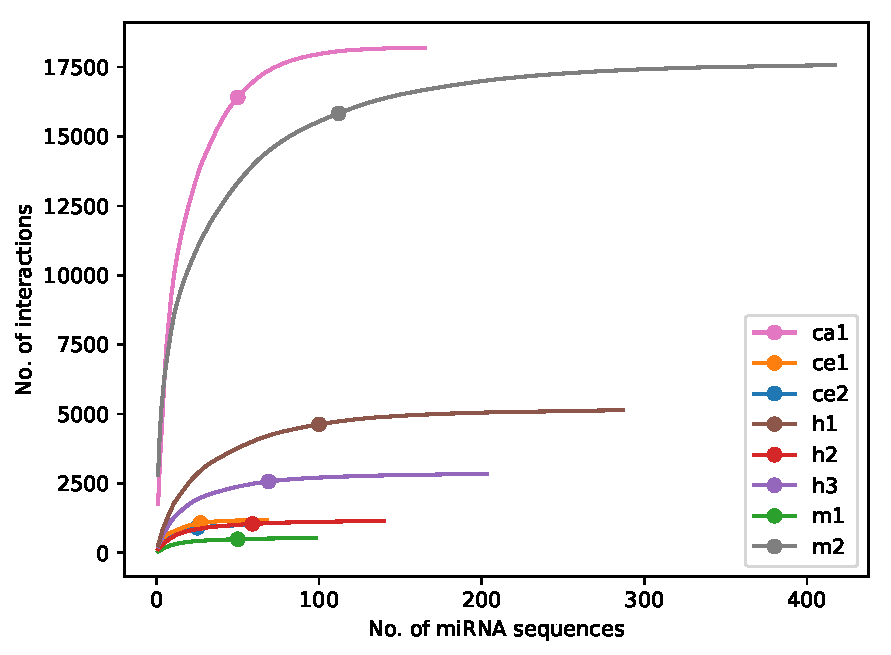
\includegraphics[width = 1\textwidth]{Results/mirna_dist.pdf}
      \label{fig:datasetplot}
      \end{figure}


\subsubsection*{Seed types and interaction strength}
We classified the interactions (i.e., the corresponding duplexes formed by the miRNA and the target site) in the datasets based on two parameters: seed type (canonical or non-canonical, see methods) and interaction strength (number of base-pairs within the duplex: weak with less than 11bp, intermediate with 11-16 base-pairs and strong with more than 16 base-pairs). We defined 6 groups (all combinations of seed type and duplex strength) and assigned each interaction to the appropriate group (Figure \ref{fig:seed_type_pos}). As can been seen in the figure, the datasets are rich and diverse, and comprise all the combinations of seed type and duplex strength. In particular, we would like to enlight 2 points: (1) In terms of seed type, majority of the interactions are non-canonical (48-70\%). (2) For both group of seed types,  majority of the interactions have intermediate and strong strength, while the weak interaction comprise only a small portion of the datasets. 
Similar analysis for the negative interactions is shown in \nameref{add:figs_tbls}, figure 1.

\begin{figure}[h!]
  \caption{\csentence{Types and characteristics of positive miRNA-target duplexes.} The percentage of miRNA-target duplexes shown in 6 groups according to the seed type [canonical and non-canonical] and to the interaction strength [weak: less than 11bp, intermediate: 11-16bp and strong: more than 16bp].}
    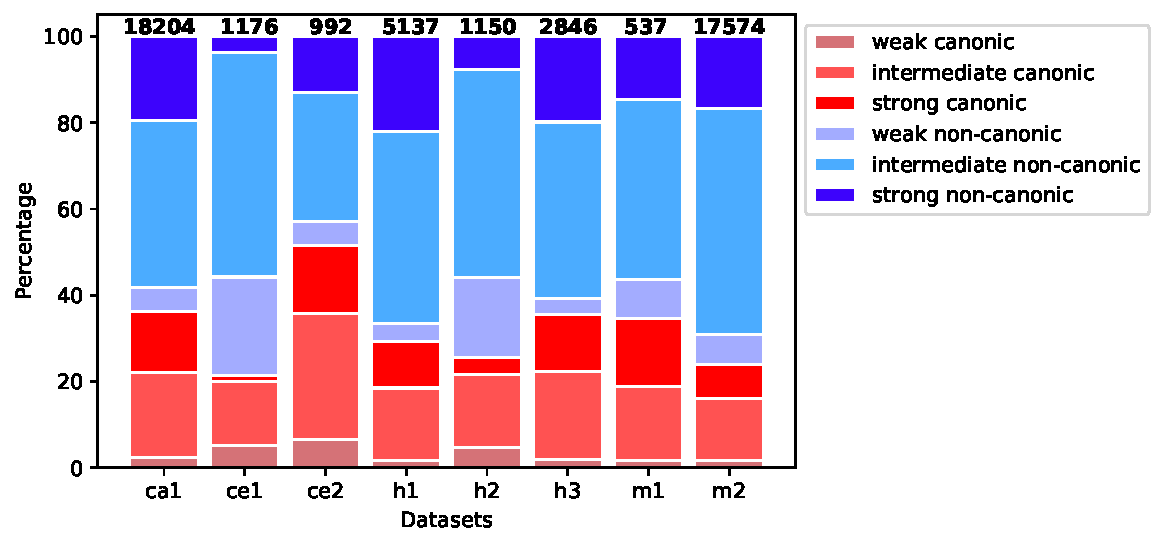
\includegraphics[width = 1\textwidth]{Results/seed_type_positive2.pdf}
      \label{fig:seed_type_pos}
      \end{figure}


% \begin{figure}[h!]
%   \caption{\csentence{Seed type and strength - negative samples}
%       bla bla bla.}
%       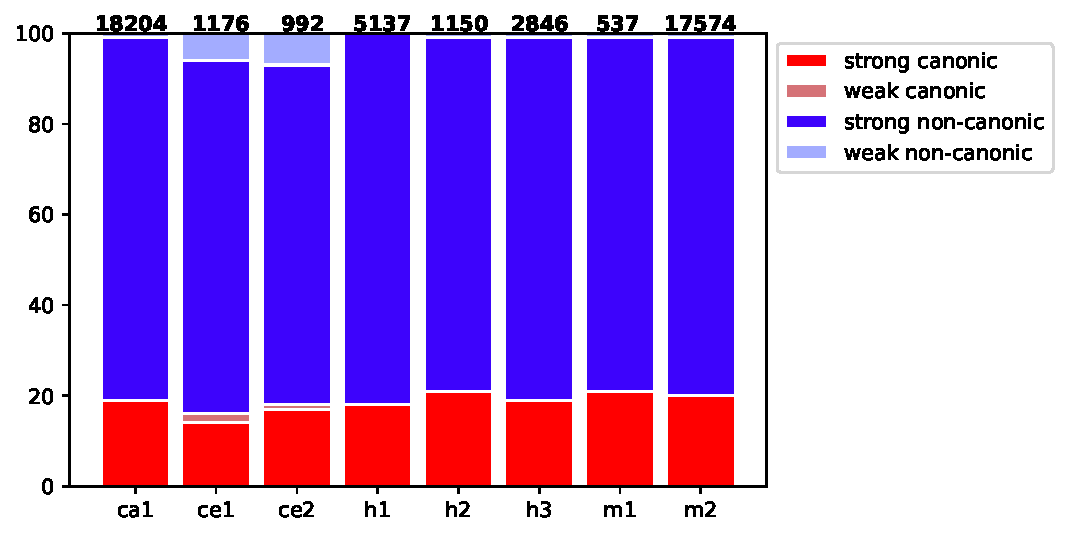
\includegraphics[width = 1\textwidth]{Results/seed_type_neg.pdf}
%       \label{fig:seed_type_neg}
%       \end{figure}


% \subsubsection*{dataset coherence test}

% Dataset coherence test measures the quality of the dataset in terms of . Here, we performed adversarial validation tests which checks the degree of similarity between the dataset samples in terms of feature distribution. It is done, by randomly splitting each dataset into two equals parts and fitted a xGBoost classifier to distinguish between the two parts. The test were run 10 times for each dataset with different random states. We used the ROC-AUC score, which ranges in value from 0 to 1: scores close to 0.5 indicate inability to distinguish between the samples which means good quality dataset. Table \ref{tbl:indataset-adv-val} shows the highest ROC-AUC score of each dataset test. All the results are close to 0.5 which confirms their validity.


% \begin{table}[h!]
% \caption{Adversarial validation AUC results}
% \label{tbl:indataset-adv-val}
% \begin{tabular}{|l|l|}
% \hline
% {} &        ROC-AUC \\ \hline
% ca1   &  0.506 (0.009) \\ \hline
% ce1 &  0.481 (0.029) \\ \hline
% ce2 &  0.523 (0.028) \\ \hline
% h1    &  0.504 (0.017) \\ \hline
% h2    &  0.535 (0.026) \\ \hline
% h3    &  0.507 (0.025) \\ \hline
% m1    &  0.532 (0.034) \\ \hline
% m2    &  0.507 (0.007) \\ \hline
% \end{tabular}
% \end{table}

\subsubsection*{Dataset visualisation}
Visualization is an important step in the analysis of high-throughput biological data and can assist in revealing hidden phenomena. However visualization is challenging when the data is represented by a large amount of features. Dimensionality reduction algorithm enables the representation of the data in 2 dimension scatter plot, and facilitates the inspection of the data by eye. MiRNA-target interactions in our study are represented by 490 features (see methods). To visualize the datasets in 2D, we performed a dimensional reduction using PCA technique (Figure \ref{fig:feature_pca}). The 2D representation explains 67\% of the variance, where percentage of variance explained by the x and the y axes are 52 and 15, respectively. 
\\Figure \ref{fig:feature_pca} reiterates the fact that there are big differences in the sizes of the datasets. In addition, there are notable differences in the 2-dimensional space spanned by each dataset: while human, cattle and mouse have points in the whole area, \textit{C.elegans} is concentrated in a narrow part of the rectangle. Moreover, a comparison of datasets of the same organism shows that a dataset composed of spontaneous chimeras from a mixture of experiments, cover less area than a dataset originating from a dedicated experiment.


% \\As can be seen in the figure, there are big differences in the sizes of the datasets.  Besides the differences in the number of interactions, there is a notable difference in the 2-dimensional space spanned by each dataset: while human, cattle and mouse have points in the whole area, \textit{C.elegans} has points in a narrow part of the rectangle. Moreover, a comparison of datasets of the same organism shows that a dataset composed of spontaneous chimeras from a mixture of experiments, cover less area than a dataset originating from a dedicated experiment.

\begin{figure}[h!]
  \caption{\csentence{Datasets presented in 2D.} Each point represents a single interaction after a dimensional reduction of its feature space using PCA. X and Y axes are the first and the second component of the PCA respectably.}
       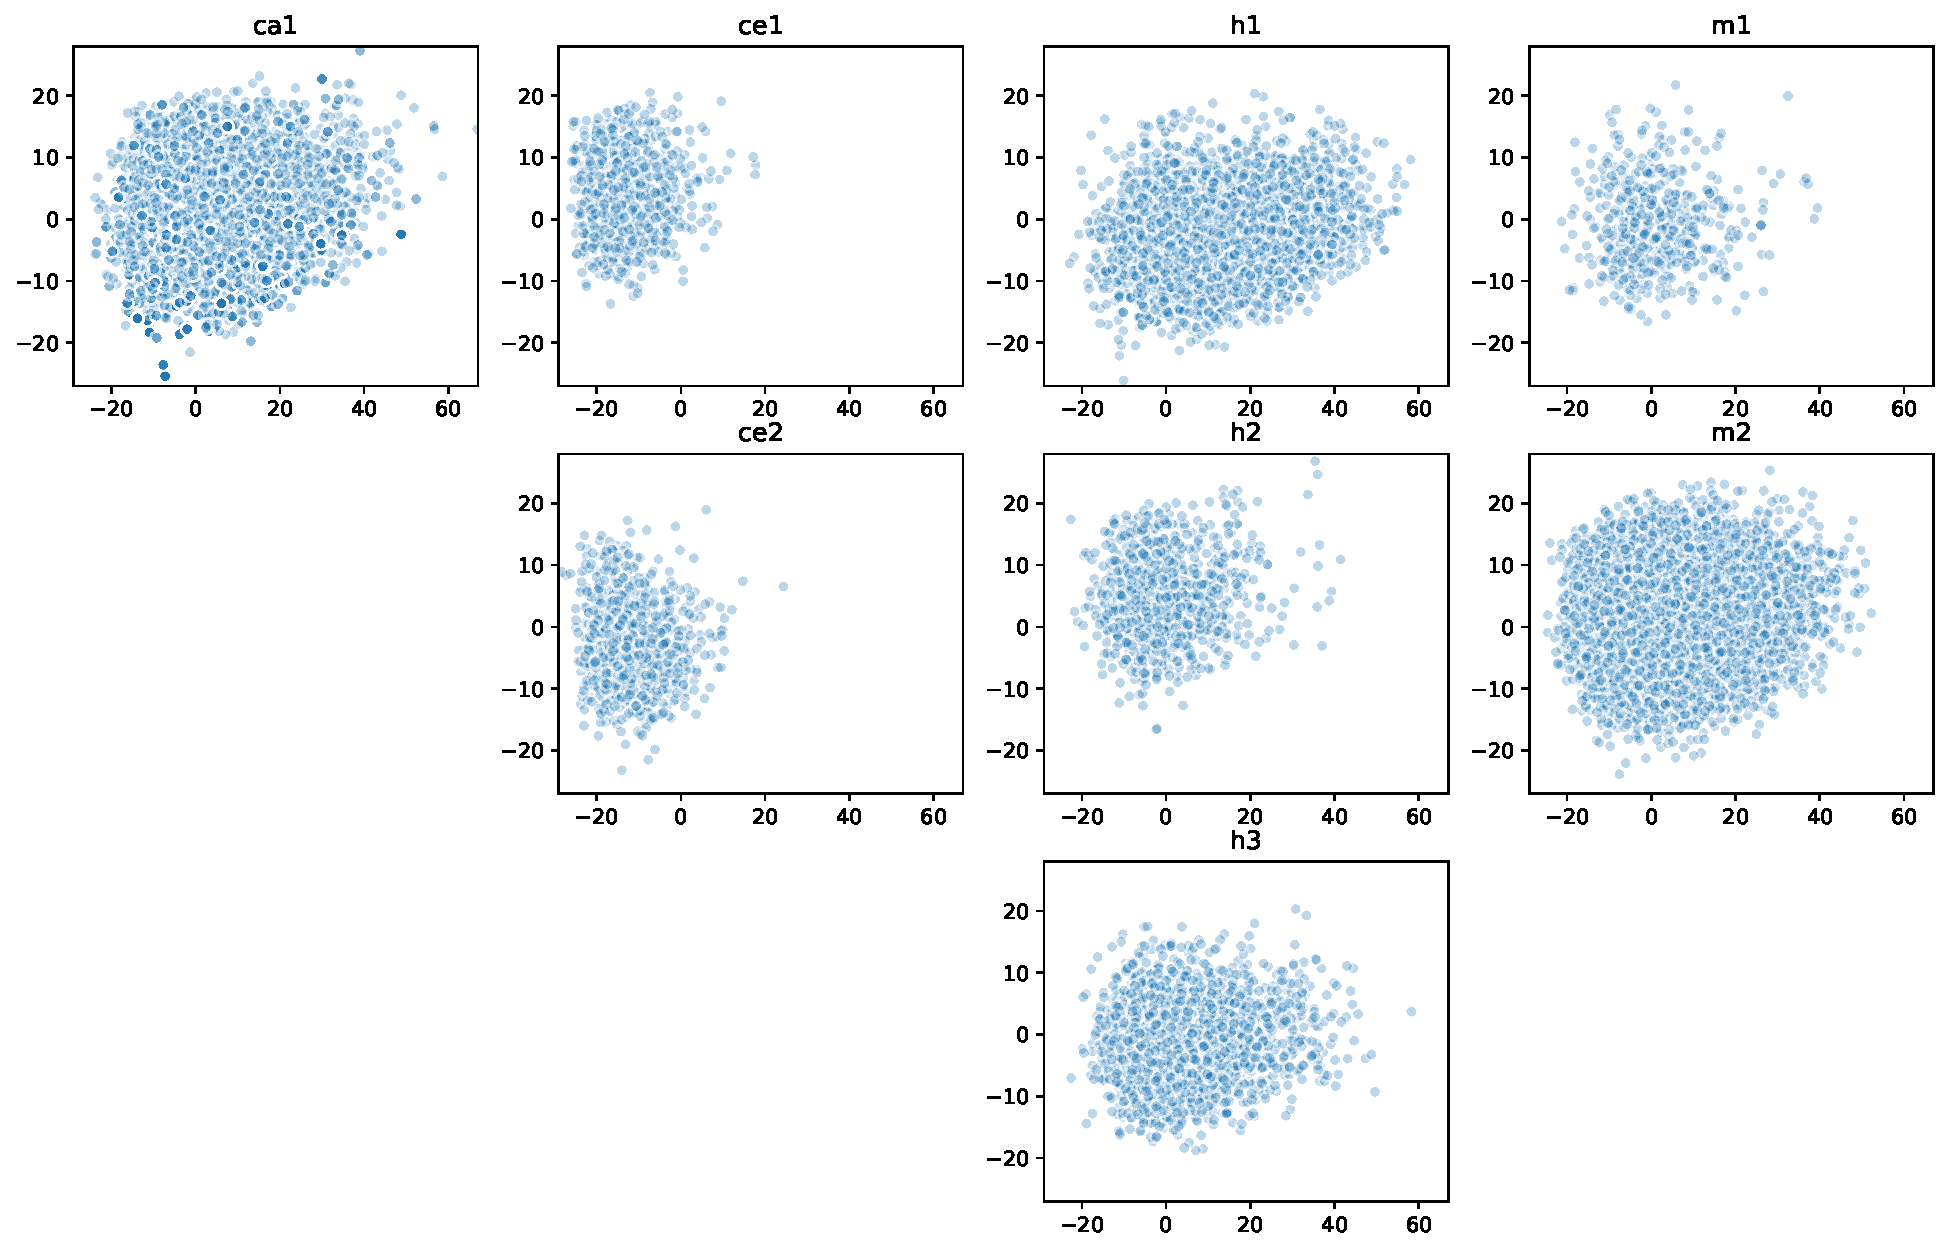
\includegraphics[width = 1\textwidth]{Results/features_pca_with_resample.pdf}
      \label{fig:feature_pca}
      \end{figure}


\subsection*{In-dataset analysis} \label{nameref:indataset}
In this section, we evaluated the performance of machine-learning based binary classifiers to correctly predict miRNA-mRNA interactions within the same dataset. 
We first conducted a set of experiments with different types of machine learning classifiers. Second, we did an in-depth analysis of the best preforming classifier including performance measurements and estimation of the top important features.

\subsubsection*{Evaluation of different machine learning methods} \label{sec:evaluation_different_ML}
We tested the performance of machine-learning based classifiers to correctly classify miRNA-target interactions. We trained 6 widely used classifiers on the training set, and measured their performance in classification of the testing set as shown in Table \ref{tab:self_summary}. xGBoost classifier achieved the best results across all datasets. 
Previous published machine learning based approaches mainly focused on the human dataset designated as h1 in table \ref{tbl:dataset_description}. We compared the results of our classifiers with previous reports and saw that the results are comparable in the achieved accuracy (\nameref{add:figs_tbls}, table 1). 

\begin{table}[h!]
\caption{In dataset prediction: accuracy performance of different machine learning methods. The cells contain the average and the STD (in brackets) results acquired from 20 models trained and evaluates on different training and testing splits.}
\label{tab:self_summary}
\begin{tabular}{|l|l|l|l|l|l|l|}
\hline
Dataset & xGBoost & RF & KNeighbors & SGD & SVM & logit \\ \hline
ca1                               & \begin{tabular}[c]{@{}l@{}}0.937 \\ (0.002)\end{tabular} & \begin{tabular}[c]{@{}l@{}}0.885 \\ (0.004)\end{tabular} & \begin{tabular}[c]{@{}l@{}}0.828 \\ (0.003)\end{tabular} & \begin{tabular}[c]{@{}l@{}}0.797 \\ (0.033)\end{tabular} & \begin{tabular}[c]{@{}l@{}}0.895 \\ (0.003)\end{tabular} & \begin{tabular}[c]{@{}l@{}}0.836 \\ (0.004)\end{tabular} \\ \hline
ce1                               & \begin{tabular}[c]{@{}l@{}}0.889 \\ (0.014)\end{tabular} & \begin{tabular}[c]{@{}l@{}}0.833 \\ (0.019)\end{tabular} & \begin{tabular}[c]{@{}l@{}}0.768 \\ (0.019)\end{tabular} & \begin{tabular}[c]{@{}l@{}}0.798 \\ (0.045)\end{tabular} & \begin{tabular}[c]{@{}l@{}}0.841 \\ (0.015)\end{tabular} & \begin{tabular}[c]{@{}l@{}}0.843 \\ (0.014)\end{tabular} \\ \hline
ce2                               & \begin{tabular}[c]{@{}l@{}}0.891 \\ (0.016)\end{tabular} & \begin{tabular}[c]{@{}l@{}}0.858 \\ (0.018)\end{tabular} & \begin{tabular}[c]{@{}l@{}}0.768 \\ (0.019)\end{tabular} & \begin{tabular}[c]{@{}l@{}}0.819 \\ (0.034)\end{tabular} & \begin{tabular}[c]{@{}l@{}}0.862 \\ (0.012)\end{tabular} & \begin{tabular}[c]{@{}l@{}}0.847 \\ (0.016)\end{tabular} \\ \hline
h1                                & \begin{tabular}[c]{@{}l@{}}0.824 \\ (0.007)\end{tabular} & \begin{tabular}[c]{@{}l@{}}0.769 \\ (0.008)\end{tabular} & \begin{tabular}[c]{@{}l@{}}0.731 \\ (0.007)\end{tabular} & \begin{tabular}[c]{@{}l@{}}0.746 \\ (0.011)\end{tabular} & \begin{tabular}[c]{@{}l@{}}0.795 \\ (0.007)\end{tabular} & \begin{tabular}[c]{@{}l@{}}0.770 \\ (0.007)\end{tabular} \\ \hline
h2                                & \begin{tabular}[c]{@{}l@{}}0.904 \\ (0.007)\end{tabular} & \begin{tabular}[c]{@{}l@{}}0.869 \\ (0.011)\end{tabular} & \begin{tabular}[c]{@{}l@{}}0.857 \\ (0.009)\end{tabular} & \begin{tabular}[c]{@{}l@{}}0.860 \\ (0.03)\end{tabular}  & \begin{tabular}[c]{@{}l@{}}0.879 \\ (0.009)\end{tabular} & \begin{tabular}[c]{@{}l@{}}0.892 \\ (0.009)\end{tabular} \\ \hline
h3                                & \begin{tabular}[c]{@{}l@{}}0.835 \\ (0.007)\end{tabular} & \begin{tabular}[c]{@{}l@{}}0.769 \\ (0.009)\end{tabular} & \begin{tabular}[c]{@{}l@{}}0.744 \\ (0.009)\end{tabular} & \begin{tabular}[c]{@{}l@{}}0.752 \\ (0.034)\end{tabular} & \begin{tabular}[c]{@{}l@{}}0.805 \\ (0.007)\end{tabular} & \begin{tabular}[c]{@{}l@{}}0.795 \\ (0.010)\end{tabular} \\ \hline
m1                                & \begin{tabular}[c]{@{}l@{}}0.847 \\ (0.015)\end{tabular} & \begin{tabular}[c]{@{}l@{}}0.795\\ (0.016)\end{tabular}  & \begin{tabular}[c]{@{}l@{}}0.758 \\ (0.022)\end{tabular} & \begin{tabular}[c]{@{}l@{}}0.760 \\ (0.038)\end{tabular} & \begin{tabular}[c]{@{}l@{}}0.819 \\ (0.019)\end{tabular} & \begin{tabular}[c]{@{}l@{}}0.800 \\ (0.019)\end{tabular} \\ \hline
m2                                & \begin{tabular}[c]{@{}l@{}}0.900 \\ (0.004)\end{tabular} & \begin{tabular}[c]{@{}l@{}}0.826 \\ (0.004)\end{tabular} & \begin{tabular}[c]{@{}l@{}}0.797 \\ (0.004)\end{tabular} & \begin{tabular}[c]{@{}l@{}}0.798 \\ (0.017)\end{tabular} & \begin{tabular}[c]{@{}l@{}}0.873\\ (0.004)\end{tabular}  & \begin{tabular}[c]{@{}l@{}}0.833 \\ (0.004)\end{tabular} \\ \hline
\end{tabular}
\end{table}


% \begin{table}[h!]
% \caption{The accuracy performance of different tools and methods, on human datasets, taken from deepMirTar.
% }
% \label{tab:existingmethods}
% \begin{tabular}{lll|l|l|}
% \cline{1-2} \cline{4-5}
% \multicolumn{1}{|l|}{\textbf{Methods}} & \multicolumn{1}{l|}{\textbf{ACC}} & \textbf{} & \textbf{Machine learning alg.} & \textbf{ACC}    \\ \cline{1-2} \cline{4-5} 
% \multicolumn{1}{|l|}{Miranda}          & \multicolumn{1}{l|}{0.6592}       &           & DT                             & 0.8139 (0.0137) \\ \cline{1-2} \cline{4-5} 
% \multicolumn{1}{|l|}{RNAhybrid}        & \multicolumn{1}{l|}{0.6988}       &           & BNB                            & 0.7570 (0.0098) \\ \cline{1-2} \cline{4-5} 
% \multicolumn{1}{|l|}{PITA}             & \multicolumn{1}{l|}{0.4981}       &           & LR                             & 0.8491 (0.0117) \\ \cline{1-2} \cline{4-5} 
% \multicolumn{1}{|l|}{TargetScan v7.0a} & \multicolumn{1}{l|}{0.5801}       &           & RF                             & 0.8811 (0.0090) \\ \cline{1-2} \cline{4-5} 
% \multicolumn{1}{|l|}{TarPmiR}          & \multicolumn{1}{l|}{0.7446}       &           & MLP                            & 0.8990 (0.0099) \\ \cline{1-2} \cline{4-5} 
% \multicolumn{1}{|l|}{DeepMirTar (SdA)} & \multicolumn{1}{l|}{0.9348}       &           & CNN-1D                         & 0.8886 (0.0145) \\ \cline{1-2} \cline{4-5} 
%                                       &                                   &           & CNN-2D                         & 0.8765 (0.0169) \\ \cline{4-5} 
% \end{tabular}
% \end{table}

% \item[1] TPR: true positive rate (Sensitivity)
% \item[2] TNR: true negative rate (Specificity)
% \item[3] PPV: Precision or positive predictive value (Precision)
% \item[4] NPV: Negative predictive value
% \item[5] FPR: false positive rate (Fall out)
% \item[6] FNR: False negative rate
% \item[7] FDR: False discovery rate
% \item[8] ACC: Overall accuracy


\subsubsection*{In-depth analysis of the xGBoost performance}
We next sought to perform an in-depth performance analysis of the xGBoost classifier since it achieved the highest accuracy across all datasets (Table \ref{tab:self_summary}). Therefore, we calculated 8 widely used performance metrics including accuracy (ACC), sensitivity (TPR: true positive rate), specificity (TNR: true negative rate), precision (PPV: positive predictive value), negative predictive value (NPV) and the rates of false positives (FPR), false negatives (FNR) and false discoveries (FDR) (Table \ref{tab:measurementinfo}). We choose these 8 measurements in order to verify that the classifier is balanced and has no bias to one class or to one type of error. As can been seen from the table, both the rate true detection (TPR and TNR) and the rate of miss-detection (FPR and FNR) are in the same range, indicating that all the 8 classifiers are balanced.


% both the rate true detection (TPR and TNR) f the true positives and negatives, and the rate of false positives and negatives are in the same range, indicating that all the 8 classifiers are balanced.

\begin{table}[h!]
\caption{xGBoost performance measurements. }
\label{tab:measurementinfo}
\begin{tabular}{|l|l|l|l|l|l|l|l|l|}
\hline
Dataset & TPR                                                    & TNR                                                   & PPV                                                      & NPV                                                      & FPR                                                      & FNR                                                      & FDR                                                      & ACC                                                      \\ \hline
ca1     & \begin{tabular}[c]{@{}l@{}}0.834\\ (0.014)\end{tabular}  & \begin{tabular}[c]{@{}l@{}}0.862\\ (0.024)\end{tabular}  & \begin{tabular}[c]{@{}l@{}}0.866\\ (0.027)\end{tabular}  & \begin{tabular}[c]{@{}l@{}}0.828\\ (0.017)\end{tabular}  & \begin{tabular}[c]{@{}l@{}}0.138\\ (0.024)\end{tabular}  & \begin{tabular}[c]{@{}l@{}}0.165 \\ (0.014)\end{tabular} & \begin{tabular}[c]{@{}l@{}}0.134 \\ (0.027)\end{tabular} & \begin{tabular}[c]{@{}l@{}}0.847 \\ (0.015)\end{tabular} \\ \hline
ce1     & \begin{tabular}[c]{@{}l@{}}0.884 \\ (0.02)\end{tabular}  & \begin{tabular}[c]{@{}l@{}}0.899 \\ (0.019)\end{tabular} & \begin{tabular}[c]{@{}l@{}}0.901 \\ (0.02)\end{tabular}  & \begin{tabular}[c]{@{}l@{}}0.881 \\ (0.023)\end{tabular} & \begin{tabular}[c]{@{}l@{}}0.101 \\ (0.019)\end{tabular} & \begin{tabular}[c]{@{}l@{}}0.116 \\ (0.02)\end{tabular}  & \begin{tabular}[c]{@{}l@{}}0.099 \\ (0.02)\end{tabular}  & \begin{tabular}[c]{@{}l@{}}0.891 \\ (0.016)\end{tabular} \\ \hline
ce2     & \begin{tabular}[c]{@{}l@{}}0.890\\ (0.018)\end{tabular}  & \begin{tabular}[c]{@{}l@{}}0.889 \\ (0.014)\end{tabular} & \begin{tabular}[c]{@{}l@{}}0.889 \\ (0.015)\end{tabular} & \begin{tabular}[c]{@{}l@{}}0.89 \\ (0.019)\end{tabular}  & \begin{tabular}[c]{@{}l@{}}0.111 \\ (0.014)\end{tabular} & \begin{tabular}[c]{@{}l@{}}0.110 \\ (0.018)\end{tabular} & \begin{tabular}[c]{@{}l@{}}0.111 \\ (0.015)\end{tabular} & \begin{tabular}[c]{@{}l@{}}0.889\\ (0.014)\end{tabular}  \\ \hline
h1      & \begin{tabular}[c]{@{}l@{}}0.823 \\ (0.011)\end{tabular} & \begin{tabular}[c]{@{}l@{}}0.849 \\ (0.009)\end{tabular} & \begin{tabular}[c]{@{}l@{}}0.854 \\ (0.011)\end{tabular} & \begin{tabular}[c]{@{}l@{}}0.816 \\ (0.015)\end{tabular} & \begin{tabular}[c]{@{}l@{}}0.151 \\ (0.009)\end{tabular} & \begin{tabular}[c]{@{}l@{}}0.177 \\ (0.011)\end{tabular} & \begin{tabular}[c]{@{}l@{}}0.146 \\ (0.011)\end{tabular} & \begin{tabular}[c]{@{}l@{}}0.835 \\ (0.007)\end{tabular} \\ \hline
h2      & \begin{tabular}[c]{@{}l@{}}0.816 \\ (0.008)\end{tabular} & \begin{tabular}[c]{@{}l@{}}0.833 \\ (0.008)\end{tabular} & \begin{tabular}[c]{@{}l@{}}0.838 \\ (0.009)\end{tabular} & \begin{tabular}[c]{@{}l@{}}0.811 \\ (0.01)\end{tabular}  & \begin{tabular}[c]{@{}l@{}}0.167 \\ (0.008)\end{tabular} & \begin{tabular}[c]{@{}l@{}}0.184 \\ (0.008)\end{tabular} & \begin{tabular}[c]{@{}l@{}}0.162 \\ (0.009)\end{tabular} & \begin{tabular}[c]{@{}l@{}}0.824 \\ (0.007)\end{tabular} \\ \hline
h3      & \begin{tabular}[c]{@{}l@{}}0.886 \\ (0.012)\end{tabular} & \begin{tabular}[c]{@{}l@{}}0.924 \\ (0.011)\end{tabular} & \begin{tabular}[c]{@{}l@{}}0.928 \\ (0.012)\end{tabular} & \begin{tabular}[c]{@{}l@{}}0.881 \\ (0.014)\end{tabular} & \begin{tabular}[c]{@{}l@{}}0.076 \\ (0.011)\end{tabular} & \begin{tabular}[c]{@{}l@{}}0.114 \\ (0.012)\end{tabular} & \begin{tabular}[c]{@{}l@{}}0.072 \\ (0.012)\end{tabular} & \begin{tabular}[c]{@{}l@{}}0.904 \\ (0.007)\end{tabular} \\ \hline
m1      & \begin{tabular}[c]{@{}l@{}}0.932 \\ (0.004)\end{tabular} & \begin{tabular}[c]{@{}l@{}}0.943 \\ (0.004)\end{tabular} & \begin{tabular}[c]{@{}l@{}}0.943 \\ (0.004)\end{tabular} & \begin{tabular}[c]{@{}l@{}}0.931 \\ (0.004)\end{tabular} & \begin{tabular}[c]{@{}l@{}}0.057 \\ (0.004)\end{tabular} & \begin{tabular}[c]{@{}l@{}}0.068 \\ (0.004)\end{tabular} & \begin{tabular}[c]{@{}l@{}}0.057 \\ (0.004)\end{tabular} & \begin{tabular}[c]{@{}l@{}}0.937 \\ (0.002)\end{tabular} \\ \hline
m2      & \begin{tabular}[c]{@{}l@{}}0.891 \\ (0.003)\end{tabular} & \begin{tabular}[c]{@{}l@{}}0.909 \\ (0.005)\end{tabular} & \begin{tabular}[c]{@{}l@{}}0.911 \\ (0.006)\end{tabular} & \begin{tabular}[c]{@{}l@{}}0.888 \\ (0.003)\end{tabular} & \begin{tabular}[c]{@{}l@{}}0.091 \\ (0.005)\end{tabular} & \begin{tabular}[c]{@{}l@{}}0.109 \\ (0.003)\end{tabular} & \begin{tabular}[c]{@{}l@{}}0.089 \\ (0.006)\end{tabular} & \begin{tabular}[c]{@{}l@{}}0.900 \\ (0.004)\end{tabular} \\ \hline
\end{tabular}
\begin{tablenotes}\footnotesize
\item[1] TPR: true positive rate (Sensitivity)
\item[2] TNR: true negative rate (Specificity)
\item[3] PPV: Precision or positive predictive value (Precision)
\item[4] NPV: Negative predictive value
\item[5] FPR: false positive rate (Fall out)
\item[6] FNR: False negative rate
\item[7] FDR: False discovery rate
\item[8] ACC: Overall accuracy
\end{tablenotes}

\end{table}

% \textit{
% TPR: true positive rate (Sensitivity)
% TNR: true negative rate (Specificity)
% PPV: Precision or positive predictive value (Precision)
% NPV: Negative predictive value
% FPR: false positive rate (Fall out)
% FNR: False negative rate
% FDR: False discovery rate
% ACC: Overall accuracy
% }
%   # Sensitivity, hit rate, recall, or true positive rate
%     "TPR" : TP / (TP + FN),
%     # Specificity or true negative rate
%     "TNR" : TN / (TN + FP),
%     # Precision or positive predictive value
%     "PPV" : TP / (TP + FP),
%     # Negative predictive value
%     "NPV" : TN / (TN + FN),
%     # Fall out or false positive rate
%     "FPR" : FP / (FP + TN),
%     # False negative rate
%     "FNR" : FN / (TP + FN),
%     # False discovery rate
%     "FDR" : FP / (TP + FP),
%     # Overall accuracy
%     "ACC" : (TP + TN) / (TP + FP + FN + TN),



\subsubsection*{Random split control}
In the above analysis, the splitting of the dataset into the training and testing sets was done in a way that preserves the miRNA distribution in both sets (stratified split). To assess how this type of split affects the classifier performance, we repeated the analysis with the xGBoost classifier, but this time used a random split strategy (control split) to generate the training and testing sets. Our results showed that there is almost no difference between the results achieved with the stratified and the control split method. The control accuracy results is shown in \nameref{add:figs_tbls}, table 2.


% In order to verify that these split does not bias the results, we run a random split method as a control and show that there is almost no difference between the tested and the control results (supplementary file XXX). 
% The accuracy results of the xGBoost classifier on the random split set shown in table \ref{tab:randomsplitacc} 
% \begin{table}[h!]
% \caption{Control results: xGBoost accuracy performance on random split.}
% \label{tab:randomsplitacc}
% \begin{tabular}{|l|l|}
% \hline
% Dataset            & XGBoost acc   \\ \hline
% ca1   & 0.938 (0.004) \\ \hline
% ce1 & 0.891 (0.013) \\ \hline
% ce2 & 0.89 0(0.012) \\ \hline
% h1    & 0.832 (0.006) \\ \hline
% h2    & 0.920 (0.013) \\ \hline
% h3    & 0.849 (0.008) \\ \hline
% m1    & 0.848 (0.011) \\ \hline
% m2    & 0.897 (0.006) \\ \hline
% \end{tabular}
% \end{table}

\subsubsection*{Top important features of each dataset}
We use the actual number of features in order to describe the interactions. Here, we would like to analyze which are the top important features of each dataset, what are the relative score between them and the degree of overlap of the top features between different datasets. xGBoost classifier reports a list of 5 feature importance metrics: weight, gain, cover, total gain and total cover. We extracted the 5 metrics for all 20 train-test splits of each dataset and calculated their mean and standard deviation (see \nameref{add:feature importance}).
For depth analysis, we used the gain metric which reflects, for each feature, its contribution to the model. For each dataset, we sorted in descending order, the average features' gain score over all 20 runs, and plot the curves of all the datasets together.
% For each dataset, we sorted in descending order,the average feature's gain score over the 20 runs,  features from the top important feature and plot them together.
Figure \ref{fig:feature_importance}a reveals that the gain score is decaying very fast. The 6 top features are significantly stronger relative to the rest (Figure \ref{fig:feature_importance} b). We extracted the top 6 features from each dataset into a unified list. The list resulted in a total of 16 features (out of the maximum length of 48),  indicating that there are many shared features among the datasets. We next extracted the gain values of these 16 features from all the datasets and normalized them to the range of (0, 100). We then ordered the features by their mean gain across all datasets (Table \ref{tab:feature_importance}). Notably, features related to the seed region (marked as bold in the table), comprise half of the features in the table. This emphasize the role of the seed region in the formation of miRNA-mRNA interactions. % We marked features related to the seed region, which are half of the feature in the table. 

The described analysis is limited due to the variance of the gain between different splits of the same dataset. Even though, it enlights the common features across datsets and the importance of the seed features.



% \begin{table}[h!]
% \caption{Feature importance}
% \label{tab:featureimportance}
% \begin{tabular}{|l|l|l|l|l|l|l|l|l|l|}
% \hline
%                                                                 & ca1   & ce1    & ce2    & h1     & h2     & h3     & m1     & m2    & mean               \\ \hline
% {\color[HTML]{FE0000} miRNAPairingCount\_Seed\_GU}              & 0.15  & 2.55   & 0.6    & 2.45   & 4.4    & 0.0    & 12.9   & 0.4   & 2.93125            \\ \hline
% {\color[HTML]{3166FF} miRNAMatchPosition\_1}                    & 1.05  & 3.1    & 4.2    & 0.75   & 9.35   & 4.05   & 15.45  & 0.6   & 4.81875 \\ \hline
% {\color[HTML]{FE0000}miRNAPairingCount\_Total\_GU}                                    & 2.45  & 43.45  & 7.1    & 0.25   & 22.7   & 1.25   & 5.9    & 4.6   & 10.9625            \\ \hline
% {\color[HTML]{32CB00} Energy\_MEF\_Duplex}                      & 6.9   & 11.65  & 61.85  & 20.75  & 0.2    & 8.65   & 5.85   & 2.0   & 14.73125 \\ \hline
% {\color[HTML]{643403} MRNA\_Target\_G\_comp}                    & 11.85 & 4.2    & 95.2   & 14.2   & 4.05   & 4.05   & 0.7    & 3.1   & 17.16875           \\ \hline
% {\color[HTML]{38FFF8} Seed\_match\_compact\_interactions\_2\_7} & 2.6   & 41.45  & 0.4    & 18.7   & 28.5   & 3.3    & 76.85  & 6.9   & 22.3375 \\ \hline
% {\color[HTML]{3166FF}miRNAMatchPosition\_9}                                           & 13.8  & 14.1   & 52.95  & 25.45  & 13.4   & 24.15  & 53.9   & 6.95  & 25.5875            \\ \hline
% {\color[HTML]{3166FF}miRNAMatchPosition\_3}                                           & 9.9   & 19.45  & 20.25  & 86.2   & 56.2   & 23.65  & 56.15  & 15.05 & 35.85625           \\ \hline
% {\color[HTML]{3166FF}miRNAMatchPosition\_5}                                           & 8.3   & 44.95  & 35.65  & 7.55   & 162.7  & 15.0   & 10.9   & 12.4  & 37.18125  \\ \hline
% {\color[HTML]{3166FF}miRNAMatchPosition\_2}                                           & 18.75 & 15.8   & 3.6    & 87.85  & 61.2   & 18.25  & 58.75  & 50.6  & 39.35              \\ \hline
% {\color[HTML]{FE0000}miRNAPairingCount\_Seed\_GC}                                   & 29.4  & 61.3   & 14.05  & 5.1    & 49.35  & 27.45  & 122.7  & 12.4  & 40.21875  \\ \hline
% {\color[HTML]{3166FF}miRNAMatchPosition\_6                                           & 31.95 & 85.2   & 65.8   & 21.75  & 102.75 & 16.5   & 57.2   & 17.05 & 49.775             \\ \hline
% {\color[HTML]{643403} MRNA\_Target\_GG\_comp}                                         & 3.75  & 100.55 & 113.8  & 16.0   & 204.25 & 4.8    & 1.1    & 4.85  & 56.1375  \\ \hline
% {\color[HTML]{3166FF}miRNAMatchPosition\_4}                                           & 16.8  & 1.3    & 11.85  & 27.7   & 54.8   & 15.75  & 318.0  & 10.95 & 57.14375           \\ \hline
% {\color[HTML]{3166FF}miRNAMatchPosition\_7}                                           & 35.55 & 60.75  & 24.45  & 74.55  & 82.45  & 63.05  & 145.3  & 19.65 & 63.21875           \\ \hline
% {\color[HTML]{FE0000}miRNAPairingCount\_Seed\_AU}                                    & 7.85  & 100.25 & 73.15  & 88.0   & 134.25 & 27.6   & 80.65  & 24.75 & 67.0625            \\ \hline
% {\color[HTML]{FE0000}miRNAPairingCount\_X3p\_bulge\_nt}                               & 112.2 & 6.7    & 213.55 & 3.0    & 8.5    & 64.2   & 173.6  & 29.7  & 76.43125           \\ \hline
% {\color[HTML]{3166FF}miRNAMatchPosition\_11}                                          & 16.1  & 50.55  & 160.1  & 129.8  & 69.5   & 60.0   & 143.1  & 36.65 & 83.225             \\ \hline
% {\color[HTML]{38FFF8} Seed\_match\_compact\_start  }                                   & 29.15 & 25.65  & 74.7   & 97.7   & 83.65  & 125.25 & 191.95 & 68.45 & 87.0625            \\ \hline
% {\color[HTML]{FE0000}miRNAPairingCount\_X3p\_AU}                                     & 70.7  & 76.65  & 252.9  & 63.6   & 73.75  & 75.75  & 105.8  & 27.7  & 93.35625           \\ \hline
% {\color[HTML]{38FFF8} Seed\_match\_compact\_A    }                                     & 22.05 & 19.8   & 18.0   & 55.5   & 359.25 & 141.95 & 120.9  & 17.75 & 94.4  \\ \hline
% {\color[HTML]{FE0000}miRNAPairingCount\_X3p\_GC}                                      & 80.85 & 63.3   & 75.4   & 25.9   & 76.25  & 104.75 & 242.5  & 90.85 & 94.975  \\ \hline
% {\color[HTML]{3166FF}miRNAMatchPosition\_12}                                          & 61.8  & 183.4  & 49.55  & 64.0   & 84.55  & 67.6   & 259.55 & 20.55 & 98.875             \\ \hline
% {\color[HTML]{32CB00}Energy\_MEF\_local\_target\_normalized}                       & 19.25 & 214.15 & 201.7  & 120.85 & 147.65 & 43.75  & 9.3    & 46.55 & 100.4 \\ \hline
% {\color[HTML]{643403} MRNA\_Target\_C\_comp }                                         & 107.5 & 68.0   & 84.6   & 93.5   & 218.4  & 142.55 & 24.6   & 65.85 & 100.625            \\ \hline
% \end{tabular}
% \end{table}


% \begin{table}[h!]
% \caption{Feature importance. The table shows the union of the top 6 features of each dataset, yielding 16 features at total.}
% \label{tab:feature_importance}
% \begin{tabular}{|l|l|l|l|l|l|l|l|l|l|}
% \hline
% \textbf{Feature/Dataset}                                   & \textbf{ca1} & \textbf{ce1} & \textbf{ce2} & \textbf{h1} & \textbf{h2} & \textbf{h3} & \textbf{m1} & \textbf{m2} & \textbf{mean} \\ \hline
% {\ul \textbf{miRNAPairingCount\_Seed\_GU}}                 & 225          & 25           & 51           & 25          & 23          & 77          & 12          & 172         & 76            \\ \hline
% {\ul \textbf{miRNAMatchPosition\_1}}                       & 142          & 23           & 18           & 63          & 14          & 23          & 11          & 147         & 55            \\ \hline
% miRNAPairingCount\_Total\_GU                               & 94           & 20           & 17           & 89          & 11          & 41          & 15          & 47          & 42            \\ \hline
% \textit{\textbf{Seed\_match\_compact\_interactions\_2\_7}} & 95           & 9            & 53           & 11          & 10          & 28          & 6           & 31          & 30            \\ \hline
% Energy\_MEF\_Duplex                                        & 29           & 13           & 6            & 9           & 58          & 14          & 15          & 90          & 29            \\ \hline
% MRNA\_Target\_G\_comp                                      & 26           & 21           & 6            & 10          & 21          & 25          & 42          & 64          & 27            \\ \hline
% MRNA\_Target\_GG\_comp                                     & 67           & 6            & 5            & 11          & 4           & 23          & 33          & 45          & 24            \\ \hline
% \textit{\textbf{miRNAMatchPosition\_4}}                    & 19           & 29           & 11           & 9           & 6           & 12          & 1           & 21          & 13            \\ \hline
% \textit{\textbf{miRNAMatchPosition\_5}}                    & 27           & 8            & 8            & 13          & 3           & 12          & 12          & 20          & 13            \\ \hline
% miRNAPairingCount\_X3p\_bulge\_nt                          & 7            & 17           & 3            & 22          & 18          & 7           & 4           & 14          & 12            \\ \hline
% \textit{\textbf{miRNAPairingCount\_Seed\_GC}}              & 15           & 6            & 13           & 16          & 7           & 10          & 4           & 20          & 11            \\ \hline
% \textit{\textbf{miRNAMatchPosition\_2}}                    & 18           & 12           & 20           & 6           & 6           & 10          & 6           & 10          & 11            \\ \hline
% Acc\_P21\_10th                                             & 19           & 5            & 4            & 6           & 14          & 6           & 5           & 11          & 9             \\ \hline
% Energy\_MEF\_local\_target\_normalized                     & 18           & 3            & 3            & 6           & 5           & 8           & 15          & 10          & 8             \\ \hline
% miRNAPairingCount\_X3p\_GC                                 & 8            & 8            & 6            & 9           & 16          & 6           & 3           & 8           & 8             \\ \hline
% \textit{\textbf{Seed\_match\_compact\_mismatch\_inner}}    & 10           & 1            & 8            & 17          & 0           & 10          & 1           & 16          & 8             \\ \hline
% \end{tabular}
% \end{table}



\begin{table}[h!]
\caption{Feature importance. The table shows the union of the top 6 features of each dataset, yielding 16 features at total. The values in the table were scaled into the range of (0, 100). For unscaled version of the table, see \nameref{add:figs_tbls}, table 3.}
\label{tab:feature_importance}
\begin{tabular}{|l|l|l|l|l|l|l|l|l|l|}
\hline
\textbf{Feature/Dataset}                          & \textbf{ca1} & \textbf{ce1} & \textbf{ce2} & \textbf{h1} & \textbf{h2} & \textbf{h3} & \textbf{m1} & \textbf{m2} & \textbf{mean} \\ \hline
\textbf{miRNAPairingCount\_Seed\_GU}              & 100          & 87           & 95           & 29          & 40          & 100         & 28          & 100         & 72            \\ \hline
\textbf{miRNAMatchPosition\_1}                    & 63           & 79           & 34           & 70          & 25          & 30          & 27          & 85          & 52            \\ \hline
miRNAPairingCount\_Total\_GU                      & 42           & 71           & 32           & 100         & 19          & 53          & 35          & 28          & 48            \\ \hline
MRNA\_Target\_G\_comp                             & 12           & 74           & 12           & 12          & 36          & 33          & 100         & 37          & 39            \\ \hline
Energy\_MEF\_Duplex                               & 13           & 45           & 11           & 10          & 100         & 19          & 35          & 52          & 36            \\ \hline
\textbf{Seed\_match\_compact\_interactions\_2\_7} & 42           & 33           & 100          & 12          & 18          & 36          & 13          & 18          & 34            \\ \hline
MRNA\_Target\_GG\_comp                            & 30           & 21           & 10           & 12          & 7           & 30          & 79          & 26          & 27            \\ \hline
\textbf{miRNAMatchPosition\_4}                    & 8            & 100          & 21           & 10          & 11          & 16          & 2           & 12          & 22            \\ \hline
miRNAPairingCount\_X3p\_bulge\_nt                 & 3            & 60           & 6            & 25          & 32          & 9           & 9           & 8           & 19            \\ \hline
\textbf{miRNAMatchPosition\_2}                    & 8            & 42           & 37           & 7           & 11          & 13          & 15          & 6           & 17            \\ \hline
\textbf{miRNAMatchPosition\_5}                    & 12           & 27           & 14           & 14          & 6           & 15          & 29          & 12          & 16            \\ \hline
\textbf{miRNAPairingCount\_Seed\_GC}              & 7            & 22           & 24           & 18          & 12          & 13          & 11          & 12          & 15            \\ \hline
miRNAPairingCount\_X3p\_GC                        & 4            & 27           & 11           & 10          & 27          & 8           & 6           & 5           & 12            \\ \hline
Acc\_P21\_10th                                    & 9            & 19           & 7            & 6           & 25          & 7           & 12          & 7           & 11            \\ \hline
Energy\_MEF\_local\_target\_normalized            & 8            & 11           & 6            & 7           & 8           & 11          & 36          & 6           & 11            \\ \hline
\textbf{Seed\_match\_compact\_mismatch\_inner}    & 4            & 3            & 15           & 19          & 0           & 13          & 2           & 9           & 8             \\ \hline
\end{tabular}
\end{table}





\begin{figure}[h!]
    \centering
    \subfloat[Full view of datasets' feature importance]{{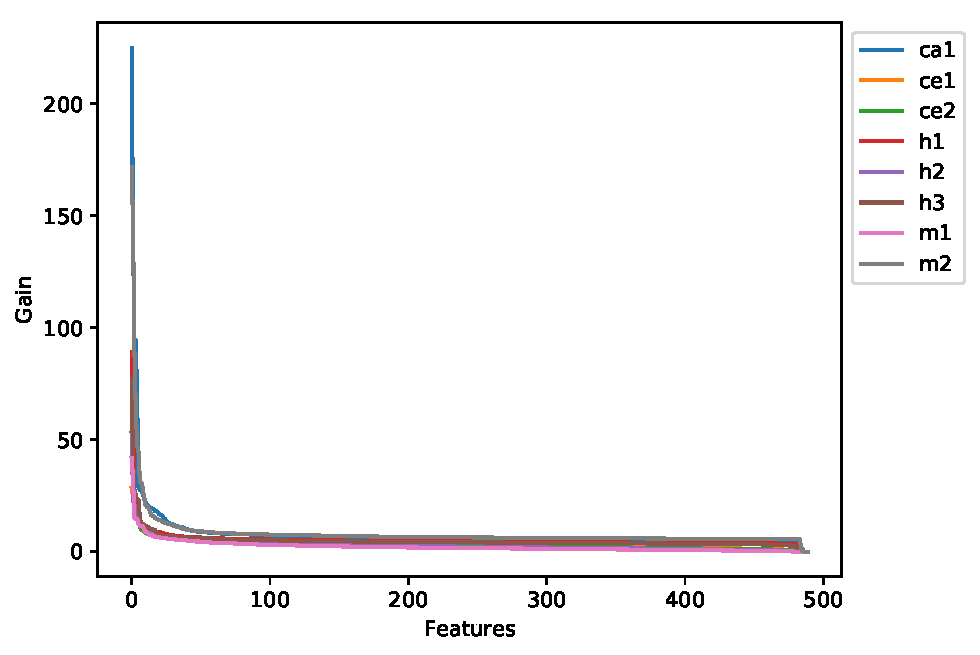
\includegraphics[width=5cm]{Results/feature_importance_full.pdf} }}%
    \qquad
    \subfloat[View of the top 20 features score]{{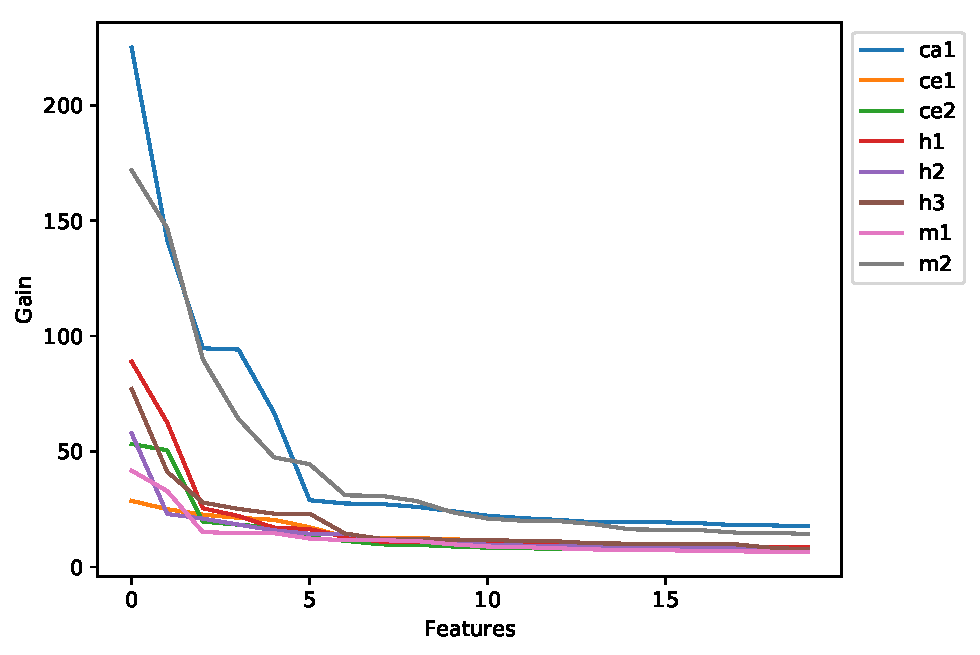
\includegraphics[width=5cm]{Results/feature_importance_zoom.pdf} }}%
    \caption{\csentence{Classifiers' feature importance}. The figures show the features' gain score. The features are descending sorted from the top feature (highest gain). Figure (a) shows a full view of the gain plot, and emphasises the gain decay.  Figure (b) is a zoomed view, focusing on the top 20 features.}%
    \label{fig:feature_importance}%
\end{figure}




% \subsection*{Target prediction between datasets}
\subsection*{Between datasets analysis}
In the previous section, we trained and optimized a dedicated classifier for each dataset, evaluated its performance and analyzed the feature importance.
% understood which are the most important features.  
In this section, we elaborate the scope of the research through analysing of relations between datasets. 
First, we used a statistical measure to calculate the distance between the datasets. Second, we evaluated the performance of each classifier in classifying the interactions in the other datasets. 
The statistics information and classification performance allow us to describe methodology for applying rules from organism to organism.

\subsubsection*{Kullback–Leibler divergence}
We hypothesized that pair of datasets, with similar characteristics, might achieve better results in classifying the interactions of each other. When we looked for a  measure for the level of similarity of pair of datasets, we took into account the fact that classification is a directed task: classifier trained on the first dataset should classify the second dataset. 
We chose the asymmetric measure Kullback–Leibler (KL) divergence which measures how one probability distribution is different from a second, reference probability distribution. We used the divergence to measure the pairwise distances between every two datasets based on their miRNA seed family distribution.

% We hypothesized that the datasets' characteristics and the level of similarity between pairs of datasets influences the classification performance of a dataset based on a classifier trained on a different dataset. Since classification is a directed task, we chose the Kullback–Leibler (KL) divergence which is an asymmetric measure. 
% The KL divergence is a measure of how one probability distribution is different from a second, reference probability distribution. We used the divergence to measure the pairwise distances between every two datasets based on their miRNA seed family distribution.
Figure \ref{fig:divergence} shows the divergence between every two dataset pairs. The divergence of a dataset with itself is zero, and usually the divergences between datasets within the same organisms are lower than the divergences between different organisms. Note that as expected due to the distance between the organisms, the divergence between \textit{C.elegans }and other datasets is significantly higher than the divergence between other pairs.

% In statistics, the Kullback–Leibler (KL) divergence is a measure of how one probability distribution is different from a second, reference probability distribution. The KL divergence is a positive, asymmetric measure that is equal to zero if and only if the distributions coincides. Here, we use the divergence to measure the distance between the miRNA seed family distribution of the training sets and the miRNA seed family distribution of the datasets it intend to predict (the testing set). 
% Figure \ref{fig:divergence} shows the divergence between all dataset pairs. The divergence of a dataset with itself is zero, and usually the divergences between datasets within the same organisms are lower than the divergences between different organisms. Note that the divergence between c.elegans and other datasets is significantly higher than the divergence between other pairs.

\todo{I would also want to know if the high divergence is because the same seed families have differences in their counts or these are totally different seeds... lets think about a way to show it, it can go to the supplement}

\begin{figure}[h!]
  \caption{\csentence{Kullback–Leibler divergence.} Each cell represents the divergence between the source and the target datasets, based on their miRNA seed family distributions}
      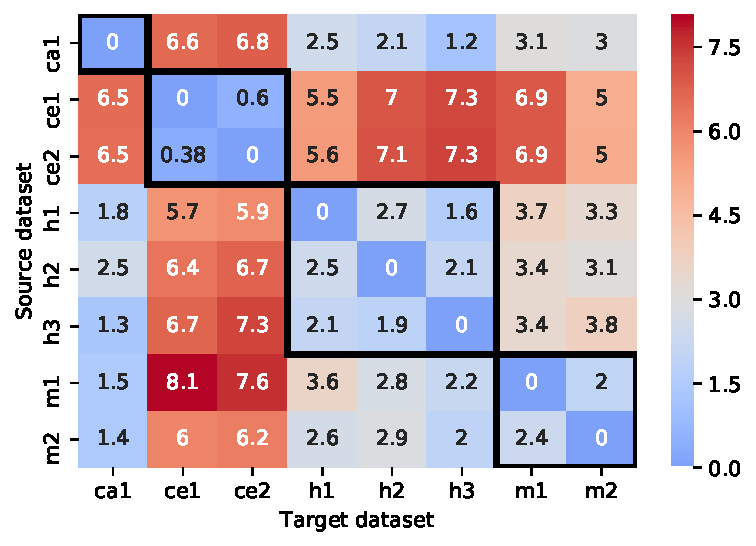
\includegraphics[width = 1\textwidth]{Results/divergence.pdf}
      \label{fig:divergence}
      \end{figure}


\subsubsection*{Classification performance between datasets}
Having the information about the datasets' characteristics, the distance between the datasets, the performance of a classifier to predict interaction derived from the same datasets it was trained on, and the the list of the shared features between datasets, we were ready to evaluated the performance cross dataset miRNA-target predictions, that is, the performance of a classifier to accurately predict interactions from datasets different from the the one it was trained on. Here, we used all datasets both as training and testing sets, and evaluated all the possible combinations. For each dataset and each training-testing split, we loaded the best xGBoost classifier found in the previous section and used it to predict the rest 7 datasets (Figure \ref{fig:crossdataset}). 
Analysis of the results show a variance in the classification performance of each pair of datasets. On one hand, the C.elegans performs well inside their own group while they are performing very bad outside it. On the other hand, most of the accuracy results between the rest organisms are above 80\%, which is similar to the accuracy performance of target-prediction algorithms from human to human. The factors influence the accuracy will be discuss in depth in discussion.

% In this section we applied the rules we have learnt from one dataset on different datasets. We used all datasets both as training and testing sets, and evaluated all the possible combinations. For each dataset, we loaded a pre-trained xGBoost model  and used it to predict the rest datasets (Figure \ref{fig:crossdataset}). The results showed in this section, support the hypothesis of the possibility to apply rules from one organism to other. The accuracy results between all the organisms despite c.elegans are above 80\%, similar to the accuracy performance of target-prediction algorithm from human to human. C.elegans perform worse in predicting other organisms or being predicted by them, with prediction performance close to random. we will suggest some explanations in discussion.


\begin{figure}[h!]
  \caption{\csentence{Cross dataset accuracy results}. Cell (i,j) represents the accuracy result of a classifier trained on the i dataset in predicting the j dataset as testing set. Each cell shows the average accuracy over the 20 best classifiers corresponding to 20 train-test splits we have (see section \nameref{sec:evaluation_different_ML}). The accuracy result for predicting the dataset itself, was taken from section \nameref{nameref:indataset}. }
      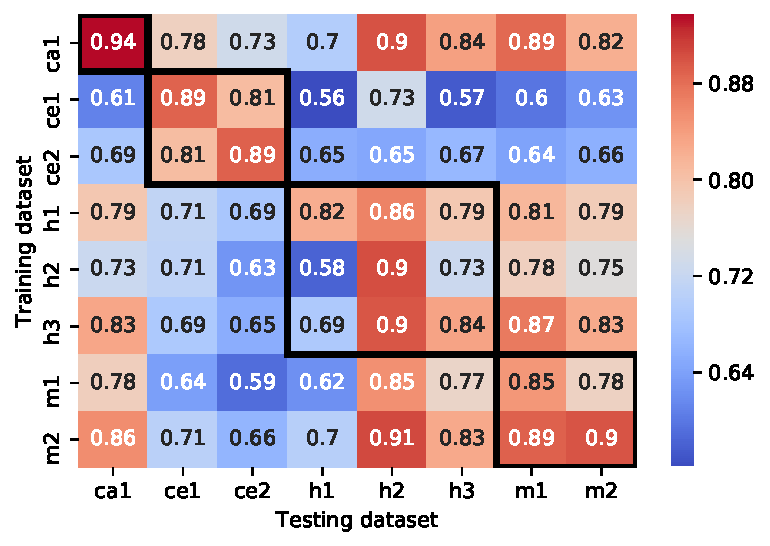
\includegraphics[width = 1\textwidth]{Results/diff_summary.pdf}
    \label{fig:crossdataset}
      \end{figure}


\section*{Discussion}
Identifying the miRNA target sites on mRNAs is a fundamental step in understanding miRNA function. miRNA target prediction tools advance this field of research and may be the basis for future applications such as biomarkers and personalized medicine. There were a notable progress in the research of this field due to the novel experimental protocols, availability of accurate data and adoption of advance machine learning methods. Classic machine learning works \todo{ref} and deep learning works \todo{ref} improved the processing pipeline, designed new features and and applied learning methods for accurate prediction. 


\subsection*{the data we used}
For a machine learning based research, the availability of large and high quality data is crucial for the succession of the research and the ability to identifying important points regarding the object we would like to study.

In the field of miRNA-target prediction, liability of isana: Discussa available high-throughput data: CLIP datasets and CLASH datasets. CLIP - reduces the search space however we still need to predict the interacting pair. CLASH and similar methods give you interacting pairs (chimeras) however the yield of these methods is relatively small. 

Previous studies trained their models on either collection of interaction from miRTarBase, CLIP data or human CLASH data. We utilized all available chimeric datasets from four organisms, generated with different methods, direct or "spontaneous" ligation, one experiment or a mix.

The available datasets are originated from variety of tissues and extracted by different biology protocols. We show that these facts are clearly reflected in the analysis. First order of analysis points on differences in the size of the datasets and the frequencies of miRNA sequences. Depth analysis points high order of differences which will discuss latter. Here, we point on 3 parameters which affect the ability to learn from dataset to dataset: Type of organism, the examined tissue and the type of experimental protocol.

\subsection*{processing pipeline}
The fact that we collected datasets from different sources and different experimental protocols, drove us to develop a processing pipeline which brought all datasets to the same standard data format. The pipeline is a powerful infrastructure which enable us, with a relatively low effort, to add data sources to our analysis. With all datasets with same format, we proceeded with exploration and analysis, in depth comparison between the datasets and performing learning tasks on them.

\subsection*{Thorough analysis of the datasets}
We found it beneficial to explore and analyze separately and together. We chose  statistical tests and visualisation methods which describe the datasets from different angles.
First, we focused on the composition of miRNA sequences and seed families within the datasets. We showed that, for each of the datsets, almost the whole of it comprises by third of the miRNA sequences or seed families.  In addition, different sets of miRNA sequences appear in different datasets, even of the same organism. Furthermore, there is a variance in the frequencies of the miRNA sequences between datasets.
The importance of the seed region was discussed in previous work... we hypothesise that this fact will impact...
We continued in examining the interaction seed type according to 2 classes: canonical and non-canonical. Majority of our interactions are non-canonical (48-70\%), which indicates that there are more factors in addition to seed interaction type which affect the possibility to interact. We analyzed the number of base-pairs in each group and found that there is almost no difference: majority of the interactions have intermediate and strong strength. \\
In the end of our analysis, we perform a 2 dimension visualization of the datasets on the same axes. The visualization reitrate some facts and gave us new insights about the datasets.





\susubsection{negative interactions}
 therefore, they represent meaningful interactions. Furthermore, it makes it hard to the classifier to distinguish between the positive and negative examples, and the classifier has to use more features and to learn complex rules.

The miRNA-target interactions, resulting from the processing pipeline, were defined as the positive examples.
The negative sets have higher percentage of non canonical seeds. This fact is expected since it is hard to achieve, randomly, duplexes with perfect seed.


\subsection{in dataset analysis}
We use a large amount of features in order to represent the interaction including high-level and low-level expert-designed features. We avoid using raw-level features, including hot encoding of the miRNA sequence since the fact that the seed families are not uniformly distributed and the negative sequence were synthetically generated with no match in the seed region, may cause the machine learning algorithm to focus on these features, and to decode the seed family rather than learning general interaction characteristics. We supply performance information with and without the raw-level features in the supplementary files. \todo {add to supp}
We used a stratify train test splits which ensured the same distribution of miRNA sequence in train and the test sets and checked it with adversarial validation technique. We generated 20 train/test sets using this algorithm with different random states. We compared the results on stratify split sets to the common random split algorithm. We are the first who does this control.
we prefer using an explainable classification algorithm rather than a black box algorithm based neural networks, in order to point on the rules and the key features the algorithm have learned. We used the xGBoost algorithm which is an high performance gradient boosting tree algorithm as our main classifier. We showed that it achieved the better performance over the statistical machine algorithm (e.g. SVM, LR) and achieved comparable results with respect to the neural nets algorithm.
We calculated variety of performance measurements showing the algorithms have no bias/tendency to any kind of classification error. \todo{add a paragraph about the feature importance}

no bias


\subsection{why tree based classifer}
We prefer a tree based estimator (rather than deep learning estimator) in order to be able to explain the model and its key features.


\subsection{features}
only the top are relevant



\subsection{relation betwenn datasets}
In order to describe the connection between the different datasets, we used the Kullback–Leibler divergence measurement which is an asymmetric measurement of how one probability distribution is different from a reference probability distribution. The result of this measurement were consistent with the evolution distance between the organisms appears in the datasets and used to explain the ability to learn form one organism to other.
Finally, we run a possible variation to learn from one organism and to apply the rules to others. We showed that there is a real potential to apply rules to other organisms. The top three factors that influence on the ability to apply rules are the evolution distance between the organisms, the coherency of the training dataset (whether it come from one or many experiments) and the size of it. We understand that the first factor reflects the similarity between rules of the train and test dataset, while the least two factors reflect the generality and quality of the learning tasks on the train dataset.


furthermore, the results much coincides with the divergence results and the evolution distance. Each groups usually better predict its members than organisms from other groups. The training dataset characteristics, such as its size and the biology procedure, found as key factors for the classifier performance: classifiers trained on large datasets predict more accurate;  classifiers trained on spontaneous-mix datasets under perform in predicting other datasets. A reasonable explanation is that small or spontaneous-mix datasets contain low diversity of samples, therefore the classifiers don't have the ability to generalize their learning.




\subsection*{Evolution distance}
We queried the \href{http://www.timetree.org} in order to understanding the evolutionary distance between two organisms, which is an estimation of the time since the two organisms last shared a common ancestor. As shown in Table \ref{tab:evolutiontime}, c.elegans has the less common with other organisms; The mouse and the human are the closet organisms among our datasets and the cattle is relatively close to them. The results are much coincides with the KL divergence results.


\begin{table}[h!]
\caption{Estimated divergence time {[}MYA{]} . Taken from http://www.timetree.org/}
\label{tab:evolutiontime}
\begin{tabular}{|l|l|l|l|}
\hline
             & Mus & Bos taurus & Caenorhabditis elegans \\ \hline
Homo sapiens & 90  & 96         & 797                    \\ \hline
Mus          &     & 96         & 797                    \\ \hline
Bos taurus   &     &            & 797                    \\ \hline
\end{tabular}
\end{table}



Most of the works dealt with a single human dataset and analyzed it individually, without any usage of information available from other experiments of same or different organisms. In this study we used machine learning techniques to examine miRNA target interactions across different organisms, both in intra-organism and inter-organism setting.

\subsection{results}

\subsection{future work}
The future potential of this research is high and include the ability to improve the prediction accuracy based on mixture of datasets and rules adopting from variety of organisms and experiments. The information coming form this research may be integrated in a less accuracy biology experiment, such as PAR-CLIP and improve their accuracy. Finally, future research also may enable us to predict, in a reasonable accuracy miRNA-target interaction without high throughput experiment at all.




\section*{Materials and methods}
\subsection*{Software packages and tools}
Code developed under this research was implemented as a Python package running on a Linux platform. It uses bioinformatics, data analysis and machine learning packages. The bioinformatics packages are ViennaRNA Package \cite{lorenz2011viennarna}, Biopython (v1.72) \cite{cock2009biopython} and NCBI Blast \cite{altschul1990basic_blast}. The data packages are pandas (v0.23.4) \cite{mckinney2010data_pandas} and numpy (v1.15.4) \cite{oliphant2006guide_numpy}. The machine learning packages are scikit-learn (v0.20.1) \cite{pedregosa2011scikit} and xGBoost (v0.81) \cite{xgboost}.

% cattle1: cattle_MDBK
% celegans1: celegans_L3
% celegans2: celegans_L2
% human1 : human_HEK293
% human2 : human_mix
% human3 : human_huh7.5
% mouse1 : mouse_mix
% mouse2 : mouse_ATCC



\subsection*{Data processing}
% \textbf{I would organize it differently. First describe everything you downloaded from where etc, then write that you have the pipeline to do the uniform format, what this format includes, and then describe the steps of the preprocessing...
% To get the miRNA sequences, fasta files were searched by the name of the miRNA ...}

We acquired eight high-throughput miRNA-target chimera datasets from four different organisms: human, mouse, cattle and worm (Table \ref{tbl:dataset_description}). The datasets' files were downloaded from the journals' websites \cite{scheel2017global, grosswendt2014unambiguous, broughton2016pairing, Helwak2014, darnell_moore2015mirna}. In addition, we downloaded miRNA sequences from miRBase (releases 17-22) \cite{kozomara2013mirbase},  3'UTR sequences from Ensembl Biomart database \cite{smedley2015biomart} and genomics information for \textit{C.elegans}, human and mouse from wormBase \cite{lee2017wormbase} and UCSC Genome Browser \cite{karolchik2004ucsc}.
The datasets were provided in different formats, containing different levels of information about the interactions. Therefore, we developed a processing pipeline to transform the datasets into a uniform format, including the following fields: metadata (interaction ID, interaction source), miRNA name and sequence, target site (the site where the interaction occurred), the corresponding 3'UTR sequence and the coordinates of the site within it.

We started the pipeline with retrieving the missing miRNA sequences by their name from miRBase. Then, we extracted the target sequences for datasets [ce2, h3, m2] based on the genomic coordinates. These target sequences are located in various mRNA region such as 5’ untranslated region (UTR), a coding sequence (CDS) or 3’ UTR. miRNA target sites located in the 3’UTRs of mRNA sequences are considered to be most functional \cite{menor2014mirmark} \todo{more REFs}. Therefore, in our analysis and experiments we discarded sites that fall outside the 3’UTRs. Since most datasets do not provide the regions containing the interactions, our next step was to obtain that information. We used Blast \cite{altschul1990basic_blast} to match the target mRNA sequences against the 3'UTRs downloaded from Ensembl Biomart database. We considered only full match results. In cases where multiple UTRs exist per a gene, we considered the longest UTR. The full 3'UTR sequences were kept for the extraction of flanking site features, as later described. Finally, we took the list of miRNA and target pairs, which are candidates for positive interactions, and examined the interaction structure. We applied ViennaRNA suite (RNAduplex 2.4.14) \cite{lorenz2011viennarna} to calculate the interaction duplex, using the miRNA sequence and the target sequences. We then classified the duplexes into canonical seed, non-canonical seed and other. Canonical seed interactions have exact Watson-Crick pairing of nts 2–7 or 3–8 of the miRNA, while non canonical seed interactions have pairing in positions 2–7 or 3–8, allowing G-U pairs and up to one bulged or mismatched nucleotide \cite{helwak2013mapping}. We allowed canonical and non-canonical seed interactions only, discarding other interactions from the analysis.
Interactions that passed all filters were designated as positive interactions and were considered for further analysis (Table \ref{tab:preprocess}).

\begin{table}[h!]
\caption{Data processing pipeline: The table describes the set of actions required to transform the datasets into a uniform format in order to serve as input for the feature extraction step. The checkmark sign (\checkmark) represents a piece of information taken directly from the paper without additional calculations.}
\label{tab:preprocess}
\begin{tabular}{|l|c|c|c|c|c|}
\hline
\textbf{Paper}       & \cite{Helwak2014} & \cite{grosswendt2014unambiguous} & \cite{scheel2017global} & 
\cite{broughton2016pairing} & \cite{darnell_moore2015mirna} \\ \hline
\textbf{Datasets}  & h1 & ce1, h2, m1 & ca1                & ce2      & h3, m2  \\ \hline
\textbf{miRNA sequence}  & \checkmark  & \checkmark           &  mirbase & mirbase  & mirbase \\ \hline
\textbf{Target sequence} & \checkmark  & \checkmark           & \checkmark                  & wormbase & UCSC genome browser  \\ \hline
\textbf{Site region}      & \multicolumn{5}{c|}{Ensembl Biomart + Blast}                                 \\ \hline
\textbf{Duplex structure}     & \multicolumn{5}{c|}{Vienna RNAduplex}                                \\ \hline
\textbf{Seed Filter} & \multicolumn{5}{c|}{Canonical and non-canonical seeds only}                \\ \hline
\end{tabular}
\end{table}

\subsection*{Generation of negative interactions}
In order to generate the negative interactions, we used a synthetic method, similarly to the method described in \cite{menor2014mirmark, john2004human, maragkakis2009accurate}. For each positive interaction appearing in the dataset, we generated a negative interaction as follows. First, we generated a mock miRNA sequence by randomly shuffling the original sequence until there is at most one match in the regions 2-7 and 3-7 between the mock miRNA and any real miRNA of the examined organism in miRBase. Next, we provided the mock miRNA and the full 3'UTR sequence as inputs to RNAduplex, which is optimized for computing the hybrid structure between a small probe sequence and a long target sequence. We repeated these two steps, until the output duplex has canonical seed or non-canonical seed. 
We managed to generate a negative interaction for each positive interaction, thus, at the end of this process we had balanced datasets.

\subsection*{Calculation of miRNA distribution} \label{miRNAdistribution}
We counted the appearance of each miRNA sequence within a dataset and used that information to generate the cumulative distribution function (CDF) showed in figure \ref{miRNAdistribution}. In order to find the 90\% value, we used the argmax function which returns the first point in the CDF which is larger than 90\%.
The seed distribution calculation was done by first clustering miRNA sequences based on their seed sequence (position 2-7), and then following the same steps described above.

\subsection*{Features} \label{methods_features}
To represent miRNA-target interactions we used 490 expert-designed features, that are classified into two categories (high-level and low-level) and five subcategories (Table \ref{tbl:feature_category}). Four of the categories (free Energy, mRNA composition, miRNA pairing and site accessibility) were adopted from \cite{wen2018deepmirtar} while the seed features group were designed in this work. For full description of the features, see Supplementary Material. \todo{add to supp} 
\\ The free energy category includes 7 features representing the minimum free energy of the miRNA alone and the miRNA duplex at different regions including site, seed, and flanking region. 
\\ The mRNA composition consists of 62 features which supply information about the target mRNA: the distance of the site from the edges of the 3'UTR (2 features), the the mRNA sequence composition within the site region (20 features) and the mRNA sequence composition of the up and down flanking region (20 features each). 
\\ The miRNA pairing consists of 38 features which describe the duplex itself, including information about base-pairs in each location of the miRNA (20 features), and total count of base-pairs, mismatches and gaps in the site region (18 features).
\\ The site accessibility features give information about the unpaired probabilities of each base to a stretch of 10 consecutive nucleotides. 
\\ In addition to above features, we designed a new representation for the seed features, which describe the base-pairing characteristics of the seed region (nt 1-8 of the miRNA). The new representation includes 13 features: 3 features describe the number of interactions in [nt1-8, nt2-7, nt3-8]; 3 features describe the number of GUs in [nt1-8, nt2-7, nt3-8]; 3 features give information about the number of mismatches (before the first match, inside the seed and after the last match in the seed region); 2 features describe the number of bulges [miRNA side, target side]; and  the last 2 features give additional metadate (start with A, index of the first base-pair).


% The site location category supply information about the distance of the site from the edges of the 3'UTR. The sequence-composition feature gives information about the duplex itself, including information about the pairs in each location, the mismatch and gaps. The site accessibility features gives information about the unpaired probabilities of each base to a stretch of 10 (ulength) consecutive nucleotides. 
% In addition to above features, we designed a new representation for the seed features, which describe the base-pairing characteristics of the seed region (nt 1-8 of the miRNA). The seed representation includes 13 features: number of interactions in [nt1-8, nt2-7, nt3-8]; number of GUs in [nt1-8, nt2-7, nt3-8]; does it start with A; the index of the first base-pair; number of mismatches before the first match, inside the seed and after the last match in the seed resign (nt1-8); number of bulges [miRNA side, target side].

% takes into account the relations and the distance between seed types. For example, "seed match 8mer" and "seed match 7mer" are relatively close, while "seed match 8mer" and "seed match 6merGU5" relatively have a loose relation and high distance. Our seed representation includes 13 features for the seed: number of interactions in [nt1-8, nt2-7, nt3-8]; number of GUs in [nt1-8, nt2-7, nt3-8]; does it start with A; the index of the first base-pair; number of mismatches before the first math, inside the seed and after the last match in the seed resign (nt1-8); number of bulges [miRNA side, target side].



\begin{table}[h!]
\caption{Feature categories that are used to represent the miRNA-target interactions}
\label{tbl:feature_category}
\begin{tabular}{|l|c|ll}
\hline
\textbf{Category}  & \multicolumn{1}{l|}{\textbf{No. of features}} & \multicolumn{1}{l|}{\textbf{Description}}                                                                                               & \multicolumn{1}{l|}{\textbf{Group}}              \\ \hline
Seed features      & 13                                        & \multicolumn{1}{l|}{Seed composition and properties.}                                                                                    & \multicolumn{1}{l|}{High-level} \\ \hline
Free Energy        & 7                                         & \multicolumn{1}{l|}{Free energy of the duplex, seed and other areas.}                                                                    & \multicolumn{1}{l|}{High-level} \\ \hline
mRNA Composition   & 62                                        & \multicolumn{1}{l|}{mRNA composition in the site and flanking areas.}                                                                           & \multicolumn{1}{l|}{High-level} \\ \hline
miRNA Pairing      & 38                                        & \multicolumn{1}{l|}{\begin{tabular}[c]{@{}l@{}}miRNA's interaction map for each nt \\ and the total interactions.\end{tabular}} & \multicolumn{1}{l|}{Low-level}  \\ \hline
Site accessibility & 370                                       & \multicolumn{1}{l|}{Unpaired probabilities of each base}                                                                                                 & \multicolumn{1}{l|}{Low-level}  \\ \hline
Total              & 490                                       &                                                                                                                                         &                                                  \\ \cline{1-2}
\end{tabular}
\end{table}

\subsection*{Dimensionality reduction using PCA}
% Visualizing the data is an important step in the analysis of high-throughput biological data. It is almost impossible to understand and to reveal phenomena in datasets with large amount of features and samples. Dimensionality reduction algorithm enables us to represent the datasets in 2 dimensions scatter plot, a representation which is easy to analyze by eye.
% Our datasets are the outputs of high-throughput experiments. The interactions in each dataset are represented by 490 features, which is impossible for visual exploration. Therefore, we used the PCA technique for reducing the number of dimensions in the datasets whilst retaining most information.
% % Principal component analysis (PCA), is a linear dimensionality reduction technique that uses Singular Value Decomposition of the data to project it to a lower dimensional space. The outputs of the PCA algorithm are orthogonal components, such as, the first principal component has the largest possible variance and each succeeding component in turn has the highest variance possible. 
Dimensionality reduction algorithm enables the representation of the data in 2 dimension scatter plot, and facilitates the inspection of the data by eye. We performed a dimensional reduction using PCA2 algorithm to transform the datasets into 2 dimension representation. 
We used the same transformer for all datasets in order to enable comparison between them. 
% A simple way to do it is by concatenating all the datasets together and applying the PCA algorithm. In our case, 
Since the datasets are with different sizes, we first over sampled them by random sampler to bring them to the size of the largest dataset. Then, we concatenated the over-sampled datasets together and fitted a PCA transformer. Finally, we applied the PCA transformer on the original datasets (without the over sampling), yielding the 2D representation of the datasets on the same vector space. 
The dimensionality reduction was done on the positive experimental interactions only.


% To be able to compare between the datasets, we would like to have the same representation for all of them. In cases of datasets with similar size, that could be done by concatenating them together and applying the PCA algorithm. In our case, since we have datasets with different sizes, we over sampled the datasets by random sampler to have equally size datasets. Then, we concatenated the over-sampled datasets together and fitted a PCA transformer. Finally, we applied the PCA transformer on the original datasets, yielding the 2D representation of the datasets on the same vector space. The dimensionality reduction was done on the positive experimental interactions only.



\subsection*{Splitting of the data into training and testing sets} \label{method:split}
Correct determination of the training and testing sets is crucial for getting reliable results. The testing set has to be large enough to yield statistically significant result, it must not contain any sample from the training set and it has to represent the dataset as a whole. 
To address these rules, we implemented a stratified random split algorithm. The algorithm ensures that each miRNA appears in the training and the testing sets at the same proportion as in the original dataset. For example, if a specific miRNA constitutes 10\% of the interactions in the original dataset, the algorithm ensures that its proportion in both the training and the testing sets is 10\%. Within the stratified split, the assignment of the interactions to training (80\%) and testing (20\%) sets is done randomly according to a random state. For miRNAs with a single interaction, we assigned the interaction to the testing set.
We repeated this process 20 times with different random states, yielding 20 training sets and 20 testing sets for each dataset.
% In order to be able to calculate the mean and the standard deviation of the results, 

In addition, for each dataset, we generated five control sets by a fully random algorithm, which does not take into account miRNA distributions. We used these sets as a reference baseline, to assess the influence of the stratified split algorithm on the results.

% \subsection*{Adversarial validation}
% We used the adversarial validation test in order to examine the coherence and the quality of the datasets. Adversarial validation test is done by randomly split the dataset into two equal groups and fitted a classifier to distinguish between them.
% % \begin{table}[h!]
% % \label{tab:my-table}
% % \begin{tabular}{|l|}
% % \hline
% % part0{[}'TARGET'{]} = 0             \\
% % part1{[}'TARGET'{]} = 1             \\
% % ROC\_AUC\_score({[}part0, part1{]}) \\ \hline
% % \end{tabular}
% % \end{table}

% % \todo{Do we need this table???}

% We use the xGBoost classifier as the classifier for the adversarial validation. For each dataset, we ran the test 10 times using different random states. The hyper parameter optimization was done by exhaustive search using sklearn GridSearchCV. The values that were used for the hyper parameter optimization are provided in supplementary files X.
% \todo{add this file}. 

\subsection*{Evaluation of different machine learning methods} \label{method_ml_methods}
We chose six different machine learning methods for the classification of miRNA-target interactions, which is a binary classification problem. We provide the accuracy results of six classifiers which are widely used for computation biology tasks: Support Vector Machine (SVM), Logistic Regression (LR), Random Forest (RF), K-Means clustering, regularized linear models with Stochastic Gradient Descent (SGD) and xGBoost\cite{xgboost} (scalable, portable and distributed gradient boosting decision trees algorithm).
% For the sixth classifier, we choose xGBoost\cite{xgboost} classifier which will be described latter.
As mentioned in subsection \nameref{method:split}, we used 25 sets of training and testing data in order to verify the model performance is not influenced by the split action. Therefore, we did the following steps 25 times, 20 times for the stratified splits and 5 times for the control splits.
First, we searched for the models' optimal hyper parameters. We performed an exhaustive search using sklearn GridSearchCV, using 4-fold cross validation, optimized for accuracy performance.  The parameters values for the hyper parameter optimization are provided in \nameref{add:hyperoptparams}. For each dataset, we performed a full training of all 6 machine learning algorithms described above. A full training of the classifiers including the hyper parameter optimization was a computationally intensive task. At total, we performed 1200 hyper parameter optimization tasks.

\begin{equation} \label{eq1}
\begin{split}
optimization \: tasks & = #classifiers * #datasets * \left (stratified\: splits + control\: splits \right ) \\
 & = 6*8*( 20 + 5 ) \\
 & = 1200
\end{split}
\end{equation}

Second, we explored the exhaustive search results and identified the set of parameters which achieved the best accuracy results. The classifiers corresponding to this set of parameters were saved and are referred as the best classifiers. At total, we have 48 best classifiers: 8 datasets * 6 machine learning algorithms.
Third, we loaded the 48 best classifiers and used them to evaluate the accuracy results on the testing set. The results shown in Table \ref{tab:self_summary} are the mean and the STD of all the train-test splits.
We continued with the xGBoost classifier for calculating detailed performance measurements and for analysis of the feature importance. We calculated 8 widely used performance metrics including accuracy, sensitivity, specificity and precision (Table \ref{tab:measurementinfo}). As before, the mean and the STD were calculated on all the train-test splits.

% The xGBoost classifier provides a scalable, portable and distributed gradient boosting decision trees algorithm. We selected the xGBoost best classifiers to calculate 8 widely used performance metrics including accuracy, sensitivity, specificity and precision (Table \ref{tab:measurementinfo}). The mean and the std of these metrics were calculated on the stratified testing sets using sklearn functions.


\subsection*{Identifying the top important features}
We used the gain metric provided by xGBoost and calculated, for each dataset, the average gain of each feature across the different 20 splits. According the gain score, we performed the following steps: First, we extracted the dominated features of each dataset. We defined the cutoff point as the point which the gain score for all the datasets were decreased in order of magnitude.  
Second, we composed a unified list of the features from all the datasets and built a table includes the gain values for the features in the list. The table's rows are the features and the columns are the 8 datasets. Next, we would like to sort the average score gain over all the datasets. However, the gain score is influenced by the dataset size. Therefore, in our third step, we normalized the feature gain score of each column: We divided each column by its maximum value and multiply it by 100. In the last step we add an average column and sorted the table descending with respect to it.


% We analyzed the average gain values and found that there is a small group of dominated features. The group of dominated is unique for each dataset, therefore, we added all the feature from all the groups into a unified group of features. Then, we built a table of the gain values from all datasets for the features in the unified group. The table enabled us to perform depth analysis of the top features across datasets.


% Given a miRNA-target interaction, our goal is to classify it to true or false interaction (i.e., binary classification). We select 6 classification algorithms for evaluation and trained them on the training set. The training and the hyper parameter optimization was done by exhaustive search using sklearn GridSearchCV. We use 4-fold cross validation, optimized the search for accuracy result.
% For the main classifier, we choose xGBoost\cite{xgboost} classifier. It provides a scalable, portable and distributed gradient boosting decision trees. We prefer a tree based estimator (rather than deep learning estimator) in order to be able to explain the model and its key features. xGBoost is relatively fast classifier, which designed to run in parallel and to utilize all the server resources. The classifier computation performance is a crucial factor due to the large number of training tasks we planed to conduct in these work. 
% As reference for xGBoost accuracy performance, we provide the results of other five classifiers which are widely used for computation biology tasks: Support vector machine classifier (SVM), Logistic regression classifier, Random forest classifier and SGD (regularized linear models with stochastic gradient descent). The values used for the hyper parameter optimization provide in supplementary files.\todo{add this file}.
% Each classifier was trained on each dataset, on all of the train-test set, yielding eventually, 1200 hyper parameter optimization (computationally intensive) tasks. 
% \begin{center}
% classifiers * datasets * (stratified splits + control sets) = \\
% = 6*8*( 20 + 5 ) = 1200
% \end{center}
% The output of the hyper parameter optimization process are the best classifiers corresponding to the methods and datasets. For the in-dataset prediction, we used the best classifiers to calculate the accuracy results on the corresponding test set.
% For the cross dataset target prediction, we show only the result of the xGBoost classifier. We use the best xGBoost classifier of a specific dataset, and use the rest dataset as test set. The test set is taken completely, without any slicing or randomization. The mean and standard deviation calculation is done on the 20 version of the best classifier derived from the train-test splits.

\subsection*{Kullback-Leibler divergence}
The Kullback-Leibler divergence is calculated on two probability distribution functions, and measures the difference and the distance between them according to equation \ref{eq:1}.

\begin{equation}
 D_{KL} \left (P ||Q \right ) = \sum_{x\in \chi }{P\left ( X \right )log\left ( \frac{P\left ( X \right )}{Q\left ( X \right )} \right )}\label{eq:1}
\end{equation}

P and Q are the miRNA seed distribution functions as explained in \ref{miRNAdistribution}. P is the distribution function of the dataset which is used to train the classifier, while Q is the distribution function of the dataset that serves as the testing set. X is the union of all the miRNA seeds that appear in the two datasets.

\subsection*{Evaluation of classification performance between datasets}
In this section, we evaluated the performance of a classifier to classify interactions derived from different data set it was trained on. We performed the evaluation tasks mentioned in this section 20 times for the different train-test splits and reported the mean and the STD of their results. 

option1: We did the evaluation in the following way: We enumerated over all the 56 possible pairs of training and testing datasets. We loaded the xGBoost classifier with the optimal parameters for the training dataset as found in section \nameref{method_ml_methods}. Then, we loaded the entire testing set (without spliting it) and evaluated the classifier performance. 

option2: We did the evaluation in the following way: We enumerated over all the 56 possible pairs of training and testing datasets:train\textsubscript{i}, test\textsubscript{j}. We loaded the xGBoost classifier with the optimal parameters for train\textsubscript{i} as found in section \nameref{method_ml_methods}. Then, we loaded the entire test\textsubscript{j} dataset (without spliting it) and evaluated the classifier performance. In cases where i=j,  we reported the result found in previous section.



% % Here, the testing set is taken completely, without any slicing or randomization. 
% The mean and standard deviation calculation is done on the 20 version of the best classifier derived from the train-test splits.






% %%%%%%%%%%%%%%%%%%%%%%%%% start of article main body
% % <put your article body there>

% %%%%%%%%%%%%%%%%
% %% Background %%
% %%
% \section*{Content}
% Text and results for this section, as per the individual journal's instructions for authors. %\cite{koon,oreg,khar,zvai,xjon,schn,pond,smith,marg,hunn,advi,koha,mouse}

% \section*{Section title}
% Text for this section \ldots
% \subsection*{Sub-heading for section}
% Text for this sub-heading \ldots
% \subsubsection*{Sub-sub heading for section}
% Text for this sub-sub-heading \ldots
% \paragraph*{Sub-sub-sub heading for section}
% Text for this sub-sub-sub-heading \ldots
% In this section we examine the growth rate of the mean of $Z_0$, $Z_1$ and $Z_2$. In
% addition, we examine a common modeling assumption and note the
% importance of considering the tails of the extinction time $T_x$ in
% studies of escape dynamics.
% We will first consider the expected resistant population at $vT_x$ for
% some $v>0$, (and temporarily assume $\alpha=0$)
% %
% \[
%  E \bigl[Z_1(vT_x) \bigr]= E
% \biggl[\mu T_x\int_0^{v\wedge
% 1}Z_0(uT_x)
% \exp \bigl(\lambda_1T_x(v-u) \bigr)\,du \biggr].
% \]
% %
% If we assume that sensitive cells follow a deterministic decay
% $Z_0(t)=xe^{\lambda_0 t}$ and approximate their extinction time as
% $T_x\approx-\frac{1}{\lambda_0}\log x$, then we can heuristically
% estimate the expected value as
% %
% \begin{eqnarray}\label{eqexpmuts}
% E\bigl[Z_1(vT_x)\bigr] &=& \frac{\mu}{r}\log x
% \int_0^{v\wedge1}x^{1-u}x^{({\lambda_1}/{r})(v-u)}\,du
% \nonumber\\
% &=& \frac{\mu}{r}x^{1-{\lambda_1}/{\lambda_0}v}\log x\int_0^{v\wedge
% 1}x^{-u(1+{\lambda_1}/{r})}\,du
% \nonumber\\
% &=& \frac{\mu}{\lambda_1-\lambda_0}x^{1+{\lambda_1}/{r}v} \biggl(1-\exp \biggl[-(v\wedge1) \biggl(1+
% \frac{\lambda_1}{r}\biggr)\log x \biggr] \biggr).
% \end{eqnarray}
% %
% Thus we observe that this expected value is finite for all $v>0$ (also see \cite{koon,khar,zvai,xjon,marg}).
% %\nocite{oreg,schn,pond,smith,marg,hunn,advi,koha,mouse}

%%%%%%%%%%%%%%%%%%%%%%%%%%%%%%%%%%%%%%%%%%%%%%
%%                                          %%
%% Backmatter begins here                   %%
%%                                          %%
%%%%%%%%%%%%%%%%%%%%%%%%%%%%%%%%%%%%%%%%%%%%%%

\begin{backmatter}

\section*{Competing interests}
  The authors declare that they have no competing interests.

\section*{Author's contributions}
    Text for this section \ldots

\section*{Acknowledgements}
  The authors would like to thank DeepMirTar team for their processing pipeline, which was partially adapted for use in this project.
 \ldots
%%%%%%%%%%%%%%%%%%%%%%%%%%%%%%%%%%%%%%%%%%%%%%%%%%%%%%%%%%%%%
%%                  The Bibliography                       %%
%%                                                         %%
%%  Bmc_mathpys.bst  will be used to                       %%
%%  create a .BBL file for submission.                     %%
%%  After submission of the .TEX file,                     %%
%%  you will be prompted to submit your .BBL file.         %%
%%                                                         %%
%%                                                         %%
%%  Note that the displayed Bibliography will not          %%
%%  necessarily be rendered by Latex exactly as specified  %%
%%  in the online Instructions for Authors.                %%
%%                                                         %%
%%%%%%%%%%%%%%%%%%%%%%%%%%%%%%%%%%%%%%%%%%%%%%%%%%%%%%%%%%%%%

% if your bibliography is in bibtex format, use those commands:
\bibliographystyle{bmc-mathphys} % Style BST file (bmc-mathphys, vancouver, spbasic).
\bibliography{bmc_article}      % Bibliography file (usually '*.bib' )
% for author-year bibliography (bmc-mathphys or spbasic)
% a) write to bib file (bmc-mathphys only)
% @settings{label, options="nameyear"}
% b) uncomment next line
%\nocite{label}

% or include bibliography directly:
% \begin{thebibliography}
% \bibitem{b1}
% \end{thebibliography}

%%%%%%%%%%%%%%%%%%%%%%%%%%%%%%%%%%%
%%                               %%
%% Figures                       %%
%%                               %%
%% NB: this is for captions and  %%
%% Titles. All graphics must be  %%
%% submitted separately and NOT  %%
%% included in the Tex document  %%
%%                               %%
%%%%%%%%%%%%%%%%%%%%%%%%%%%%%%%%%%%

%%
%% Do not use \listoffigures as most will included as separate files

\section*{Figures}
  \begin{figure}[h!]
  \caption{\csentence{Sample figure title.}
      A short description of the figure content
      should go here.}
      \end{figure}

\begin{figure}[h!]
  \caption{\csentence{Sample figure title.}
      Figure legend text.}
      \end{figure}

%%%%%%%%%%%%%%%%%%%%%%%%%%%%%%%%%%%
%%                               %%
%% Tables                        %%
%%                               %%
%%%%%%%%%%%%%%%%%%%%%%%%%%%%%%%%%%%

%% Use of \listoftables is discouraged.
%%
\section*{Tables}
\begin{table}[h!]
\caption{Sample table title. This is where the description of the table should go.}
      \begin{tabular}{cccc}
        \hline
           & B1  &B2   & B3\\ \hline
        A1 & 0.1 & 0.2 & 0.3\\
        A2 & ... & ..  & .\\
        A3 & ..  & .   & .\\ \hline
      \end{tabular}
\end{table}

%%%%%%%%%%%%%%%%%%%%%%%%%%%%%%%%%%%
%%                               %%
%% Additional Files              %%
%%                               %%
%%%%%%%%%%%%%%%%%%%%%%%%%%%%%%%%%%%

\section*{Additional Files}
  \subsection*{Additional file 1} \label{add:figs_tbls}
    Figures and tables. PDF format

  \subsection*{Additional file 2}  \label{add:feature importance}
    feature_importance.xlsx
 
 \subsection*{Additional file 3}  \label{add:hyperoptparams}
   grid_search_params.yaml




\section*{Additional data files}




\begin{enumerate}
\item Additional file 1
\item feature_importance.xlsx
\item cattle\_dataset1.csv
\item celegans\_dataset1.csv
\item celegans\_dataset2.csv
\item human\_dataset1.csv
\item human\_dataset2.csv
\item human\_dataset3.csv
\item mouse\_dataset1.csv
\item mouse\_dataset2.csv
\item grid\_search\_params.yaml
\item feature importance \todo{feature importance. ask Isana if the colors are important}
\item feature description
\item random split
\item performance of raw features ???
\item dist of negative


\end{enumerate}




\end{backmatter}
\end{document}
